\chapter{Modelli collettivi}

\section{Liquid drop Model}

The liquid-drop model is a collective model.
For light nuclei the larger part of binding energy, approx 7 Mev per nucleons, lies in forming $\alpha$-cluster ($SU_4$ or wigner supermultiplet symmetry) 
Because of the short-range nature of nuclear force the binding energy to a first approx increases linearly with A.

\begin{figure}[!ht]
\centering
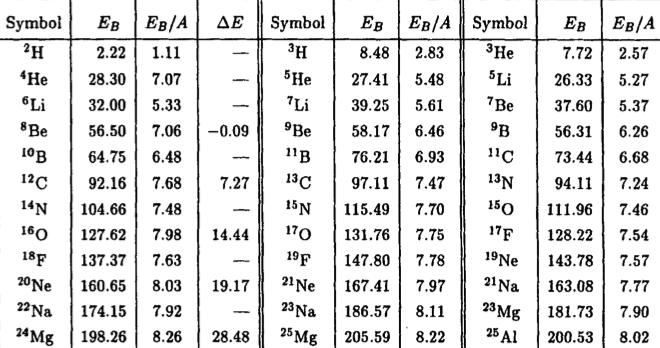
\includegraphics[width=\textwidth,height=\textheight,keepaspectratio]{lightBE}
\caption{Binding energies (MeV) for some stable light nuclei
.}
\end{figure}

Esprimo la massa del nucleo con $M(Z,N)=Zm_p+Nm_n-\frac{E_B}{c^2}$:

la formula semiempirica dice che
\begin{equation*}
E_B=a_vA-a_SA^{\frac{2}{3}}-a_C\frac{Z^2}{A^{\frac{1}{3}}}-a_A\frac{(A-2Z)^2}{A}-\delta(A,Z)
\end{equation*}

\begin{enumerate*}
\item Volume term.

Since the nucleon density is assumed constant, every individual particle will have the same number of neighbours as every other.
\begin{equation*}
a_VA\propto V
\end{equation*}

\item Surface term.

With the above explanation the nucleus is assumed infinite, but the nucleus is of a finite size, consequently those nucleons on the surface do not bind as strongly as those nearer the centre: 

surface area $\propto A^{\frac{2}{3}}$.

\begin{equation*}
a_SA^{\frac{2}{3}}
\end{equation*}

\item Coulomb term.

 For a given proton it will repel Z-1 other protons, this will occur Z times, so a Z(Z-1) term is obtained. The average distance between two protons in a nucleus is proportional the total radius of the spherical nucleus
 \begin{equation*}
-a_C\frac{Z(Z-1)}{A^{\frac{1}{3}}}
 \end{equation*}


Per ricavare $a_C$:
\begin{align*}
&E=\frac{3}{5}(\frac{1}{4\pi\epsilon_0})\frac{Q^2}{R}=\frac{3}{5}(\frac{1}{4\pi\epsilon_0})\frac{{Ze}^2}{r_0A^{\frac{1}{3}}}\\
&=\frac{3e^2Z^2}{20\pi\epsilon_0r_0A^{\frac{1}{3}}}\approx a_C\frac{Z(Z-1)}{A^{\frac{1}{3}}}\\
&a_C=\frac{3}{5}(\frac{\hbar c \alpha}{r_0})=\frac{3}{5}(\frac{R_P}{r_0})\alpha m_pc^2&\intertext{ con $R_P$ Proton Compton radius.}
\end{align*}

\item Asymmetry (kinetic) term.

Since the difference between potential energy and kinetic (hence the alternate name) energy (PE-KE) of a nucleon is the binding energy of a nucleon, the new neutron (or proton) will have less binding energy than the previous ones. Therefore an excess of one nucleon over the other would lead to less average binding energy.

\begin{equation*}
-a_{sym}\frac{(Z-N)^2}{A}
\end{equation*}

\item Pairing term

\begin{align*}
\delta(A,Z)=\left\{\begin{array}{l}-\frac{a_P}{A^{\frac{1}{2}}} \text{ Z,N even}\\0 \text{ A odd}\\+\frac{a_P}{A^{\frac{1}{2}}} \text{ Z,N odd}\end{array}\right.
\end{align*}
The nuclear mass for given odd A.
$M_A>\frac{1}{2}(M_{A-1}+M_{A+1})$:
$B_A<\frac{1}{2}(B_{A-1}+B_{A+1})$.
\end{enumerate*}

\begin{figure}[!ht]
\centering
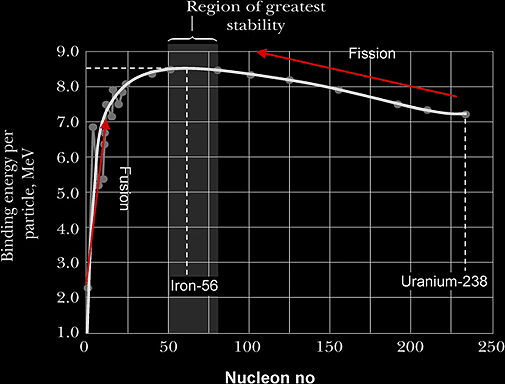
\includegraphics[width=\textwidth,height=0.5\textheight,keepaspectratio]{BE-A}
\caption{L'energia di legame per nucleone \'e circa costante per nuclei pesanti}
\end{figure}

\begin{figure}[!ht]
\centering
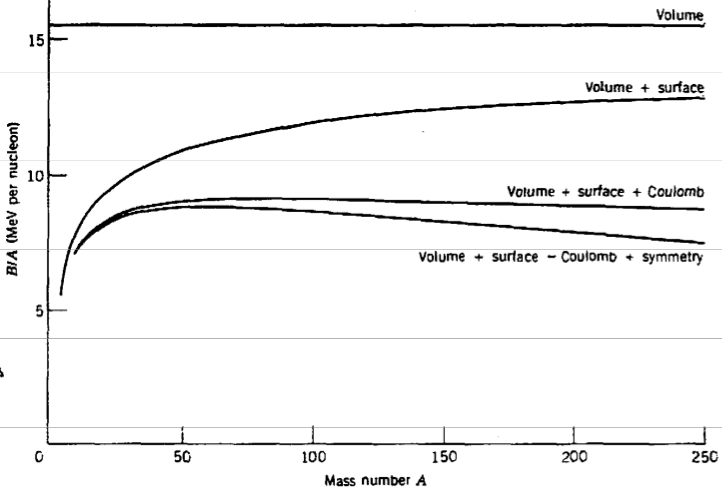
\includegraphics[width=\textwidth,height=0.5\textheight,keepaspectratio]{BEparts}
\caption{Contribution to BE per nucleon in the liquid drop model.}
\end{figure}

\section{Collective properties: Shell model problems}

\begin{figure}[!ht]
\centering
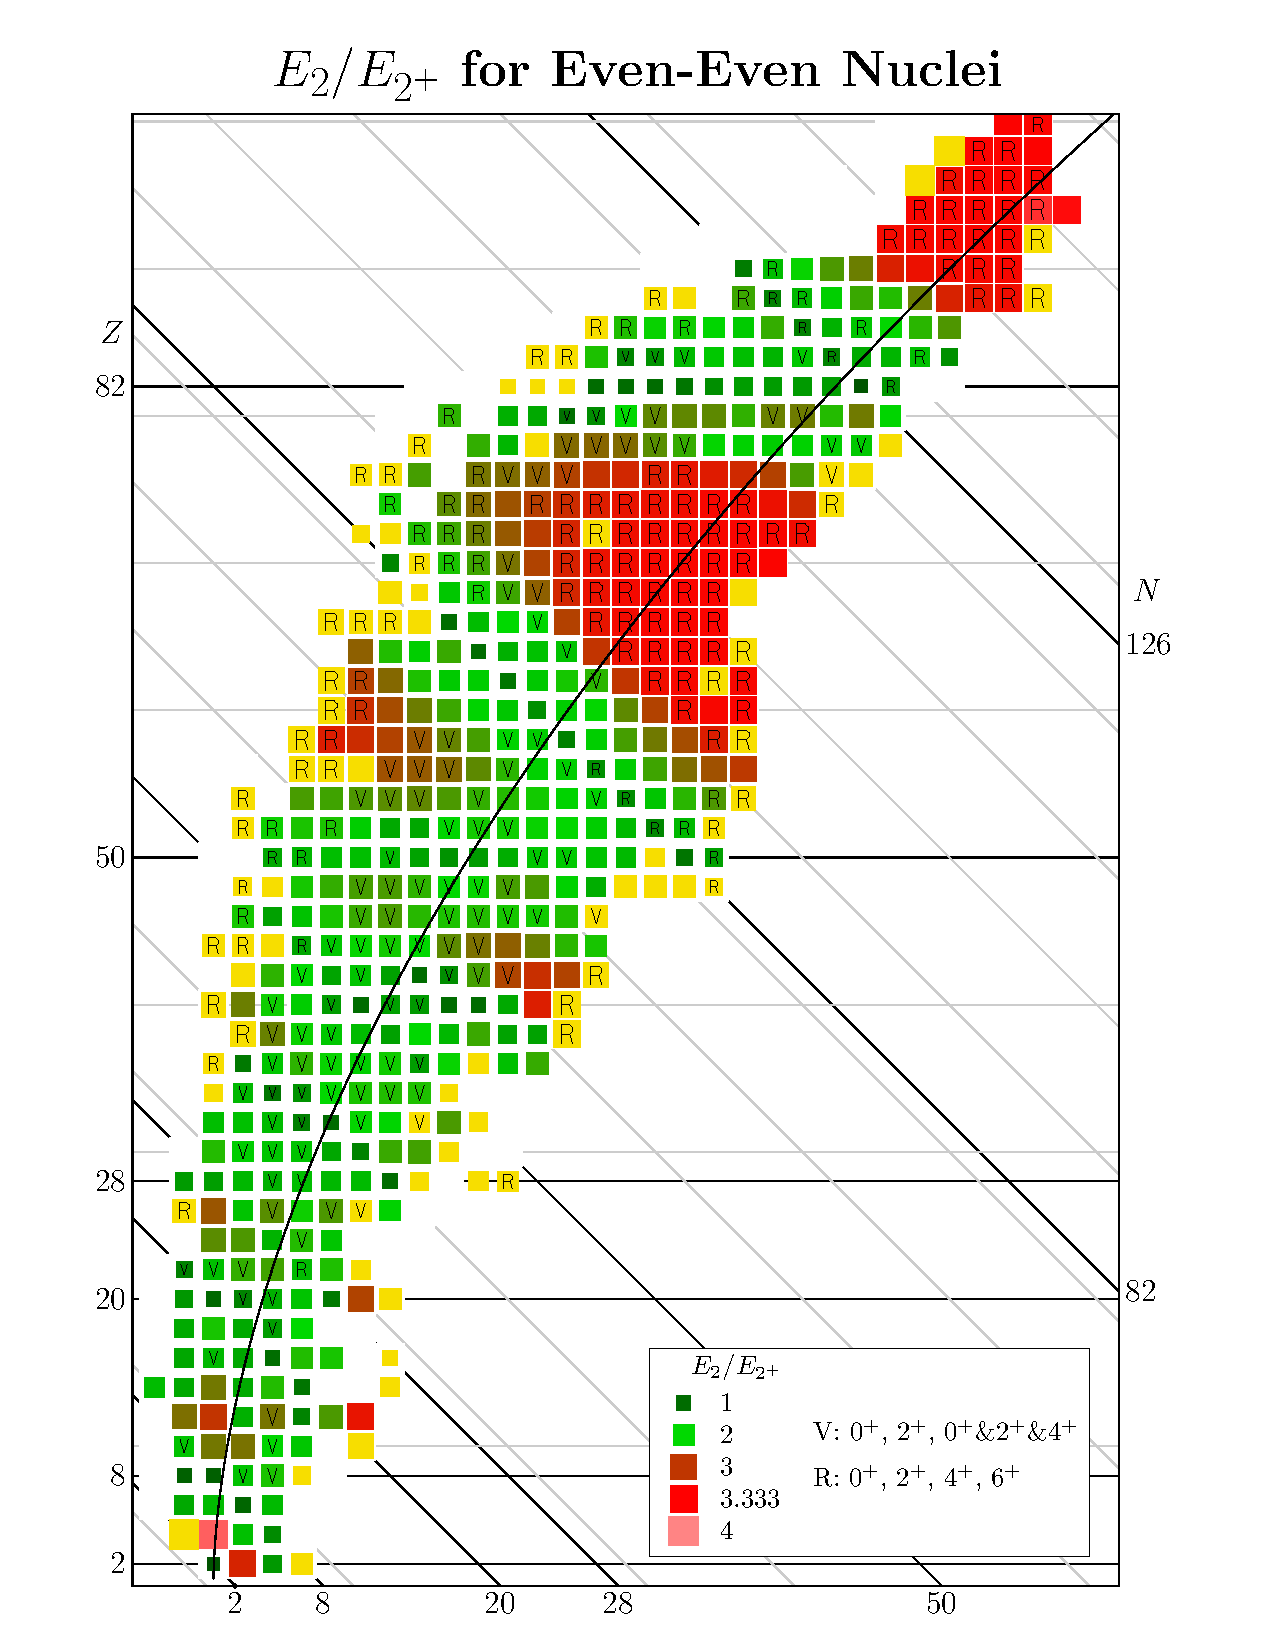
\includegraphics[width=(\textwidth-18mm),height=(\textheight-11mm),keepaspectratio]{e2e2p}
\caption{Excitation energy ratio for even-even nuclei.}
\end{figure}

\subsection{Livelli potenziale sferico}
\begin{equation*}
1s_{\frac{1}{2}},\,1p_{\frac{3}{2}},\,1p_{\frac{1}{2}},\,1d_{\frac{5}{2}},\,2s_{\frac{1}{2}},\,1d_{\frac{3}{2}},\,1f_{\frac{7}{2}},\,2p_{\frac{3}{2}},\,1f_{\frac{5}{2}},\,2p_{\frac{1}{2}},\,1g_{\frac{9}{2}}
\end{equation*}

\subsection{Excited states in even-even nuclei.}

La presenza di un livello eccitato $2^+$ con $E_{ex}\approx1.2\,MeV$, meno dell'energia necessaria per disaccoppiare 2 nucleoni, in tutti i nuclei pari-pari modellizzabili in shell ci induce a considerare la struttura collettiva.

\subsection{Momento di quadrupolo elettrico}

Per alcuni nuclei con shell quasi riempite ho momento di quadrupolo maggiore del previsto.

\begin{align*}
&^A_ZX_N\quad\text{Valence}\quad &J\quad &Q_o \quad &Q_T\\
&^{17}_8O_9 \quad+1\Pneutron \quad&\frac{5}{2} \quad&-2.6 \quad&-0.1 \\
&^{39}_{19}K_{20} \quad-1\Pproton \quad&\frac{3}{2} \quad&5.5 \quad&5 \\
&^{175}_{71}Lu_{104} \quad / \quad&\frac{7}{2} \quad&560\quad&25 \\
&^{209}_{83}Bi_{126}\quad+1\Pproton\quad&\frac{7}{2} \quad&-35\quad&-30
\end{align*}

\subsection{Energie caratteristiche}

\section{Liquid drop + shell model}

Propriet\'a collettive:
\begin{itemize*}
\item Variano con continuit\'a in funzione di m e gradualmente in funzione di A
\item Sono scarsamente influenzate dai nucleoni di valenza: in nucleoni di valenza possono contribuire alla struttura a shell che si accoppia alla struttura collettiva.
\end{itemize*}


\section{Modello vibrazionale.}

I livelli dei nuclei con $A<150$ sono trattati in termini di vibrazioni di una struttuara di equilibrio sferica.

\subsection{The classical perturbation of the surface of the drop.}

Propriet\'a armoniche sferiche

\begin{align*}
&Y_{l,m}^*=(-1)^mY_{l,-m}\\
&\int_0^{2\pi}\int_0^{\pi}Y_{lm}Y_{l'm'}^*\,d\Omega=\frac{4\pi}{(2l+1)}\delta_{ll'}\delta_{mm'}\\
&P_l(\hat{x}\cdot\hat{y})=\frac{4\pi}{2l+1}\sum_{\mu=-\lambda}^{+\lambda}Y_{lm}(\theta,\phi)Y_{lm}^*(\theta',\phi')\\
&Y_{lm}(\theta,\phi)\to Y_{lm}(\pi-\theta,\pi+\phi)=(-1)^lY_{lm}(\theta,\phi)&\intertext{questa sopra \'e la trasformazione sotto parit\'a}
\end{align*}

Piccole deformazioni

\begin{align*}
R(t)=R_{Av}+\sum_{\lambda\geq1}\sum_{\mu=-\lambda}^{\lambda}a_{\lambda\mu}(t)Y_{\lambda\mu}(\theta,\phi)&\intertext{il raggio deve essere reale:}\\
R(t)=R(t)^*\quad\Rightarrow\quad a_{\lambda\mu}=(-1)^{\mu}a_{\lambda,-\mu}
\end{align*}

Le coordinate collettive $a_{\lambda\mu}$ (tensore) definiscono la distrosione/vibrazione del nucleo rispetto allo stato fondamentale.

Modi ad alte energia
\begin{itemize*}
\item Breathing mode: $\lambda=0$, espansioni/contrazioni.
\item Dipole mode: $\lambda=1$, oscillazioni del centro di massa.
\end{itemize*}

\subsection{Equazioni fluidodinamiche: Equazione di Laplace.}

\begin{align*}
&\frac{\partial}{\partial t}\rho+\nabla\cdot(\rho\vec{v})=0\quad\text{(Continuit\'a)}\\
&\vecp{\nabla}{v}=0&\intertext{fluido irrotazionale:}\\
&\vec{v}=\nabla\phi&\intertext{$\phi$ \'e il campo scalare delle velocit\'a}
\end{align*}

Per un fluido incompressibile ottengo l'equazione di Laplace
\begin{align*}
&\nabla\cdot(\rho\vec{v})=0=\underbrace{\nabla\rho}_{0}\cdot\vec{v}+\rho\scap{\nabla}{v}\\
&\nabla^2\phi=0
\end{align*}

Soluzioni equazione Laplace
\begin{align*}
&\phi(r,\theta,\phi)=\sum_{\lambda\mu}b_{\lambda\mu}*r^{\lambda}Y_{\lambda\mu}(\theta,\phi)&\intertext{soluzione regolare in 0.}\\
&\phi(r,\theta,\phi)=\sum_{\lambda\mu}\frac{R_0^{-\lambda+2}}{\lambda}\dot{a_{\lambda\mu}}*r^{\lambda}Y_{\lambda\mu}(\theta,\phi)&\intertext{ho ricavato i coefficienti b dal confronto}\\
&v_r=\frac{\partial\phi}{\partial r}=\dot{R}
\end{align*}

Energia cinetica

\begin{align*}
T&=\frac{1}{2}\int_{Vol}v^2\,d^3r=\frac{1}{2}\int_{Vol}|\nabla\phi|^2\,d^3r=\frac{1}{2}\oint_{\Sigma}\phi^*\nabla\phi\,d^3r\\
&=\frac{1}{2}\sum_{\lambda}B_{\lambda}|\dot{a_{\lambda\mu}}|^2
\end{align*}

\subsection{Potenziali di deformazione}
Scrivo il contributo  all'energia dovuto alla tensione superficiale
\begin{align*}
&E_S^{(0)}=\sigma4\pi R_0^2=a_SA^{\frac{2}{3}}\\
&E_S=\sigma\oint\,dS=\frac{a_s}{4\pi R_0^2}\oint\,dS=\frac{1}{2}\sum_{\lambda\mu}C_{\lambda}^{(S)}|a_{\lambda\mu}|^2
\end{align*}

e all'interazione Coulombiana

\begin{align*}
&E_C^{(0)}=\frac{3}{5}\frac{(eZ)^2}{R_0}=a_C\frac{Z^2}{A^{\frac{1}{3}}}\\
&E_C=\frac{1}{2}\int\frac{\rho(\vec{r_1})\rho(\vec{r_2})}{|\vec{r_1}-\vec{r_2}|}\,d^3r_1\,d^3r_2=\frac{1}{2}\sum_{\lambda\mu}C_{\lambda}^C|a_{\lambda\mu}|^2
\end{align*}
e scrivo la perturbazione
\begin{equation*}
V=(E_S-E_S^{(0)})+(E_C-E_C^{(0)})
\end{equation*}

\subsection{Modi normali}
Definisco le coordinate e gli impulsi generalizzati
\begin{align*}
&a_{\lambda\mu}\\
&\Pi_{\lambda\mu}=B_{\lambda}\dot{a_{\lambda\mu}^*}\\
&[a_{\lambda\mu},\Pi_{\lambda'\mu'}]=i|\hbar\delta_{\lambda\lambda'}\delta_{\mu\mu'}
\end{align*}
quindi scrivo l'Hamiltoniana collettiva
\begin{align*}
H_{Coll}&=\frac{1}{2}\sum_{\lambda\mu}[B_{\lambda}|\dot{a_{\lambda\mu}}|^2+C_{\lambda}|a_{\lambda\mu}|^2]\\
&=\frac{1}{2}\sum_{\lambda\mu}[\frac{|\Pi_{\lambda\mu}|^2}{B_{\lambda}}+C_{\lambda}|a_{\lambda\mu}|^2]
\end{align*}

\subsection{Energy quantization}

Operatori creazione/distruzione

Le regole di selezione degli operatori di creazione $P^{\dag}_{\lambda\mu}$ e distruzione $P_{\lambda\mu}$ per un fonone di energia $E=\hbar\omega_{\lambda}$ e momento $\lambda$ sono
\begin{align*}
[P^{\dag}_{\lambda'\mu'},P^{\dag}_{\lambda\mu}]=[P_{\lambda'\mu'},P_{\lambda\mu}]=0\\
[P^{\dag}_{\lambda'\mu'},P^{\dag}_{\lambda\mu}]=\hbar\delta_{\lambda\lambda'}\delta_{\mu\mu'}
\end{align*}

\subsection{Fononi: infiniti oscillatori disaccoppiati}
\begin{align*}
&H_{Coll}=\sum_{\lambda\mu}\omega_{\lambda}\hbar(P^{\dag}_{\lambda\mu}P_{\lambda\mu'}+\frac{1}{2})\\
&E_{\lambda}=\hbar\omega_{\lambda}\sum_{\mu}(N_{\mu}+\frac{1}{2})=\hbar\omega_{\lambda}(N+\frac{2\lambda+1}{2})
\end{align*}

\subsection{Accoppiamento di 2 fononi: eccitazioni di quadrupolo ($\lambda=2$).}
Regole di selezione per stato di $N=2$ fononi di momento definito:

\begin{align*}
&\ket{N=2,\lambda,\mu}=\sum_{\mu',\mu''}\braket{22\lambda|\mu',\mu'',\mu}P^{\dag}_{2\mu'}P^{\dag}_{2\mu''}\ket{0}&\intertext{La funzione d'onda di bosoni identici \'e simmetrica}\\
&\ket{N=2,\lambda,\mu}=\\
&\frac{1}{2}\sum_{\mu',\mu''}[1+(-1)^{\lambda}]\braket{22\lambda|\mu',\mu'',\mu}P^{\dag}_{2\mu'}P^{\dag}_{2\mu''}\ket{0}&\intertext{tengo solo i termini pari, viste le propriet\'a di inversione dei CCG:}\\
&\braket{J_1J_2J|m_1m_2M}=(-1)^{J_1+J_2-J}\braket{J_2J_1J|m_2m_1M}
\end{align*}

\subsection{Stati eccitati vibrazionali}
\begin{equation*}
\frac{E(4^+)}{E(2^+)}\approx2
\end{equation*}

\section{Modello rotazionale}
Landau 575

Nuclei con $150<A<190$ o $A>220$ mostrano struttura tipica di rotazione di un sistema non sferico.

\subsection{Nuclei deformati: Momento di quadrupolo}
Net nuclear potential due to filled core shell not necessarily spherically symmetric.

\subsection{Bande rotazionali}

\chapter{Fenomenologia dell'\Ra-decay}

\section{Introduzione storica}

La particella $\alpha$ f\'u da prima identificata come la meno penetrante fra le emissioni di elementi naturalmente radioattivi.

In 1903 Rutherford measured their charge-to-mass ratio by deflecting \Ra particles from the decay of radium in electric and magnetic field; in 1909 Rutherford showed that \Ra were helium nuclei.

\section{Descrizione schematica}

\subsection{Decadimenti nel chart di segre}

\begin{figure}[!ht]
\centering
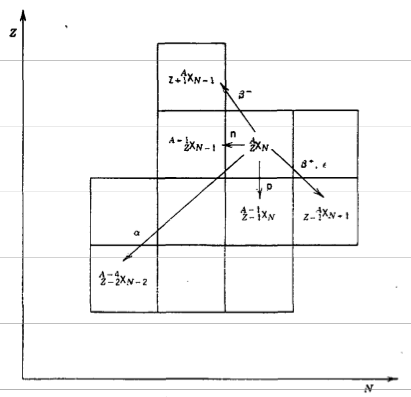
\includegraphics[width=(\textwidth-18mm),height=(\textheight-11mm),keepaspectratio]{ntrans}
\label{fig:ntrans}
\end{figure}

\begin{equation*}
^A_ZX_N\rightarrow^{A-4}_{Z-2}X'_{N-2}+\alpha+Q
\end{equation*}

\subsection{Coulomb repulsion}
 \Ra-decay is a Coulomb repulsion effect: the disruptive Coulomb force increases with size at a faster rate, $Z^2$, than does the specific nuclear binding force $\approx A$.

\subsection{Energia cinetica dei prodotti}

The kinetic energy of an \Ra-particle can be measured with a magnetic spectrometer and so the Q value of a decay can be determined:

$(m_X-m_{X'}-m_{\alpha})c^2=T_{X'}+T_{\alpha}=Q$ that is energy conservation\\ $m_Xc^2=m_{X'}c^2+T_{X'}+m_{\alpha}c^2+T_{\alpha}$, the decay will occur spontaneously only if $Q>0$.

Q value can be calculated from atomic mass tables because electrons masses cancel each other.

If the original nucleus is at rest the total linear momentum is zero, $\vec{p}_{\alpha}=\vec{p}_{X'}$, then we can the classical $T=\frac{p^2}{2m}$ since energy released is about few MeV ($T\ll mc^2$):


\begin{align*}
T_{\alpha}&=\frac{Q}{(1+\frac{m_{\alpha}}{m_{X'}})}\\
&\approx Q(1-\frac{4}{A})
\end{align*}

since usually is $A\gg4$.

Tipicamente \Ra acquista il $98\%$ dell'energia cinetica Q mentre il nucleo pi\'u pesante rincula con circa il $2\%$ dell'energia cinetica resa disponibile: per un valore tipico di $Q=5 MeV$ il nucleo rincula con un'energia cinetica di 100 KeV (is far in excess of that which binds atoms in solids). And if we know the mass of the long lived (supposed) X we can determine the mass of a short lived $X'$.

\section{Relazione di Geiger-Nuttal}

One  feature of \Ra decay, so striking that it was noticed as long ago as 1911 by Geiger and Nuttal, is that\\
\Ra emitters with large disintegration energies had short halft-life and conversely.

\begin{equation*}
\ln{\lambda}=-a_1\frac{Z}{\sqrt{Q}}+a_2
\end{equation*}

For example:

\begin{align*}
^{232}Th (1.4*10^{10} y; Q=4.08 MeV)\\
^{218}Th (1.0*10^{-7}s; Q=9.85 MeV)
\end{align*}

A factor of 2 in energy means a factor of $10^{24}$ in half-life.
 
 \begin{figure}[!ht]
\centering
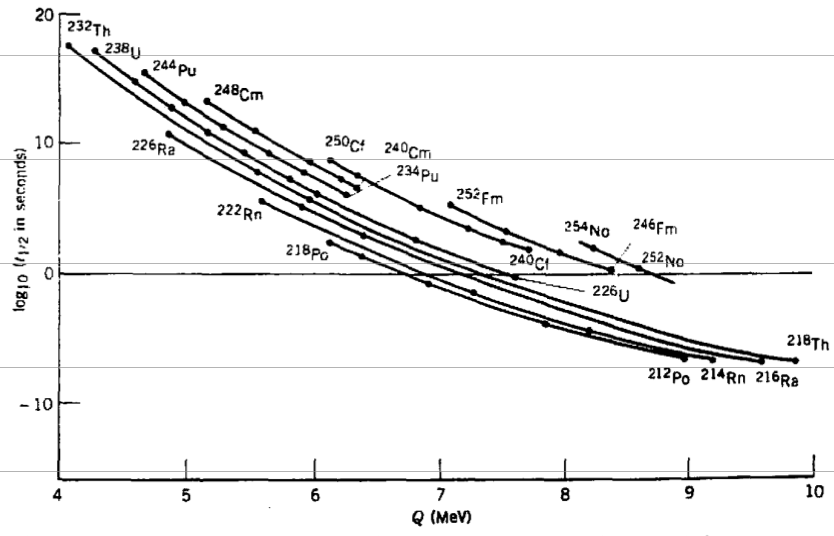
\includegraphics[width=(\textwidth-18mm),height=(\textheight-11mm),keepaspectratio]{GNplot}
\caption{\Ra-decay: Tempo di dimezzamento $\thalf$ vs Q.}
\label{fig:GNplot}
\end{figure}

Very smooth curves result if we plot only \Ra emitters with the same Z (and further if we select  only those with (N,Z) both even as in this chart; the curves for odd-even, even-odd, odd-odd nuclei are not smooth curves: their periods are 2-1000 times longer than even-even types with same Z and Q.)


\section{Stima di Q usando SEMF.}

\subsection{SEMF:}

$M(Z,N)=Zm_p+Nm_n-\frac{E_B}{c^2}$, cio\'e
\begin{align*}
M(Z,N)&=Zm_p+Nm_n-a_vA+a_SA^{\frac{2}{3}}+a_C\frac{Z^2}{A^{\frac{1}{3}}}+\\
&+a_A\frac{(A-2Z)^2}{A}+\delta(A,Z)\\
&\delta(A,Z)=\left\{\begin{array}{c}33.6*A^{-\frac{3}{4}} \text{N,Z pari}\\0 \text{A dispari}\\33.6A^{-\frac{3}{4}} \text{N,Z dispari}\\\end{array}\right.
\end{align*}


SEMF coefficients:

\begin{align*}
a_V=15.5 MeV\\
a_S=16.8 Mev\\
a_C=0.72 MeV\\
a_{Sym}=23 MeV\\
a_{pair}=34 MeV
\end{align*}

We can compare the systematic dependence of Q on A with SEMF prediction:

\begin{align*}
&Q=B(^4He)+B(Z-2,A-4)-B(Z,A)\\
&\approx28.3-4a_V+\frac{8}{3}a_SA^{-\frac{1}{3}}+4a_CZA^{-\frac{1}{3}}(1-\frac{Z}{3A})\\
&-4a_{sym}(1-2\frac{Z}{A})^2+3a_PA^{-\frac{7}{4}}&\intertext{approssimazione $A,Z\gg1$}
\end{align*}

Comparison between experimantal value and predicted.

\begin{tabular}{|l|c|c|}
\hline
Nucleus & $Q_{\text{nat}} (MeV)$ & $Q_{SEMF} (MeV)$\\
\hline
$^{226}Th$ & $6.45$ & $6.75$ \\
\hline
$^{232}Th$ & $4.08$ & $5.71$  \\
\hline
$^{220}Th$ & $8.95$ & $7.77$ \\
\hline
\end{tabular}\\

The parameter of SEMF are chosen to give rough agreement with observed binding energies across the entire range of nuclei: it' important that the SEMF gives rough agreement with the decay Q value and that it correctly gives $Q>0$ for heavy nuclei, correctly predict the decrease of Q with increasing A for a sequence of isotopes although it gives too small a change of Q with A (the formula gives $\Delta Q=-0.17 MeV/A$ while the observed average change is $\Delta Q=-0.40 MeV/A$).

 \begin{figure}[!ht]
\centering
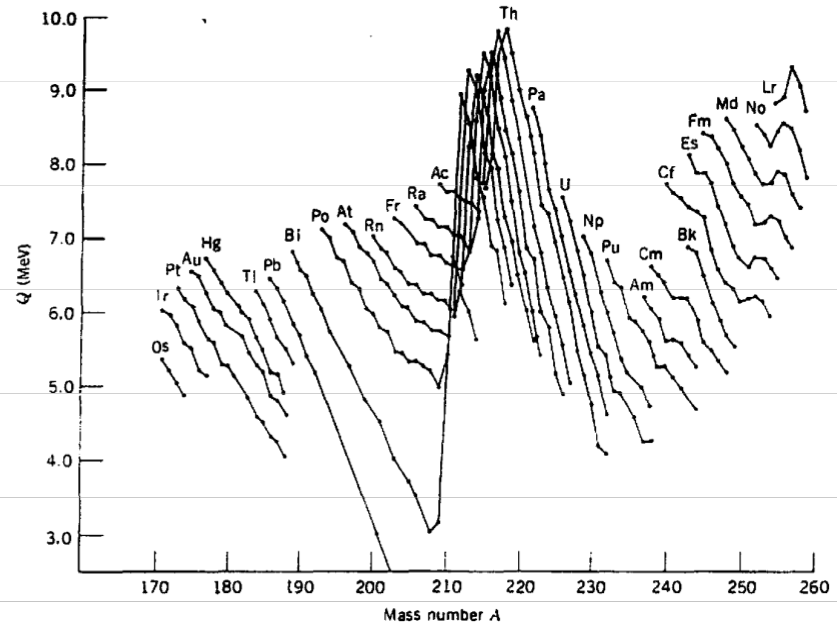
\includegraphics[width=(\textwidth-18mm),height=(\textheight-11mm),keepaspectratio]{alphaQvsA}
\caption{\Ra-decay: Q vs A}
\label{fig:alphaQvsA}
\end{figure}

Energy release in \Ra-decay for various isotopic sequences of heavy nuclei. We see the effects of the shell closures at $N=126$ ($A=212$) (large dip in data) and $Z=82$ (larger than average spacing between Po, Bi and Pb sequence).


\subsection{Soglia di instabilit\'a}
 
\begin{figure}[!ht]
\centering
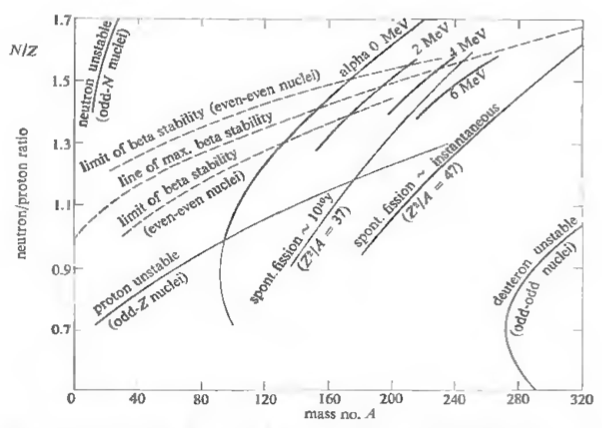
\includegraphics[width=(\textwidth-18mm),height=(\textheight-11mm),keepaspectratio]{SEMFsline}
\caption{Zone di stabilit\'a nel grafico A vs N/P ratio.}
\label{fig:SEMFsline}
\end{figure}

 \begin{figure}[!ht]
\centering
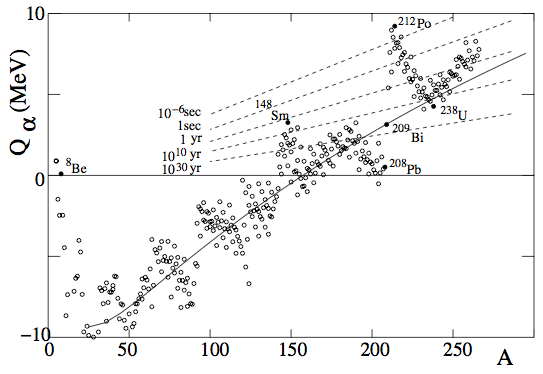
\includegraphics[width=(\textwidth-18mm),height=(\textheight-11mm),keepaspectratio]{QvsAnat}
\caption{$Q_{\alpha}$ vs. $A$ for $\beta$-stable nuclei.}
\end{figure}


The solid line shows the prediction of the semi-empirical mass formula. Because of the shell structure, nuclei just heavier than the doubly magic $^{208}Pb$ have large values of $Q_{\alpha}$ while nuclei just lighter have small values of  $Q_{\alpha}$. The dashed lines show half-lives calculated according to the Gamow formula. Most nuclei with $A>140$ are potential \Ra-emitters, though, because of the strong dependence of the lifetime on $Q_{\alpha}$, the only nuclei with lifetimes short enough to be observed are those with $A>209$ or  $A\approx148$, as well as the light nuclei $^8Be$, $^5Li$ e $^5He$.

One consequence of the strong rate dependence on $Q_{\alpha}$ is the fact that \Ra-decays are preferentially to the ground state of the daughter nucleus, since decays to excited states necessarily have smaller values of $Q_{\alpha}$.  In \Rb-decays, the
$Q_{\beta}$ dependence is weaker and many \Rb-decays lead to excited states.

\chapter{Modello di Gamow-Gurney-Condon dell'\Ra-decay}

\section{One body model: alfa preformed inside dauther nucleus}

\subsection{Barriera di potenziale rettangolare: Coefficiente di trasmissione}

Considero una barriera di potenziale rettangolare tale che le soluzioni dell'equazione di Schr\"odinger 
\begin{equation*}
\frac{d^2}{dx^2}+\frac{2m}{\hbar^2}(E-V)u=0
\end{equation*}

possano essere scelte della forma

\begin{align*}
&u_I=A_I\exp{ikx}+B_I\exp{-ikx}\quad-\infty<x<0\\
&u_{II}=A_{II}\exp{Kx}+B_{II}\exp{Kx}\quad0<x<a\\
&u_{III}=A_{III}\exp{ikx}+B_{III}\exp{-ikx}\quad a<x<+\infty&\intertext{dove ho posto:}\\
&k=\frac{\sqrt{2mE}}{\hbar}=\frac{p}{\hbar}=\frac{1}{\lambdabar}\\
&K=\frac{\sqrt{2m|E-V|}}{\hbar}
\end{align*}

Mi interessano le onde che si propagano verso $x>0$ quindi pongo $B_{III}=0$ e dalle condizioni di continuit\'a di $u$ e $\frac{du}{dx}$ ho le relazioni per $x=a$
\begin{align*}
A_{II}=\frac{A_{III}}{2}(1+\frac{ik}{K})\exp{(ik-K)a}\\
B_{II}=\frac{A_{III}}{2}(1-\frac{ik}{K})\exp{(ik+K)a}
\end{align*}
e  per $x=0$
\begin{align*}
A_I+B_I=A_{II}+B_{II}\\
A_I-B_I=(A_{II}-B_{II})\frac{K}{ik}
\end{align*}
eliminando $A_{II}$ e $B_{II}$ troviamo la relazione fra $A_I$, l'ampiezza dell'onda incidente, $B_I$ ampiezza dell'onda riflessa e $A_{III}$ ampiezza dell'onda trasmessa. 

Quando $Ka\gg1$, barriera quasi opaca, possiamo semplificare trascurando $A_{II}$ rispetto a $B_{II}$ e otteniamo $2A_I=B_{II}(1-\frac{K}{ik})=\frac{A_{III}}{2}(1-\frac{ik}{K})(1-\frac{K}{ik})\exp{(ik+K)a}$.

Determino il coefficiente di trasmissione
\begin{equation*}
T=\frac{|A_{III}|^2}{|A_I|^2}=\frac{16k^2K^2\exp{-2Ka}}{(k^2+K^2)^2}\approx\exp{2Ka}
\end{equation*}

questo da il flusso di probabilit\'a trasmesso per unit\'a di flusso incidente; mentre per la riflettivit\'a dobbiamo usare la soluzione esatta
\begin{equation*}
R=\frac{|B_I|^2}{|A_I|^2}
\end{equation*} 
Nel caso di un potenziale variabile possiamo generalizzare la formula per il coefficiente di trasmissione
\begin{equation*}
T=exp[-\frac{2}{\hbar}\int\sqrt{2m|E-V(x)|}dx]=\exp{-2G}
\end{equation*}
esteso alla regione in cui $E-V<0$, classicamente proibita.

\subsection{Dall'equazione di Schr\"oedinger al fattore di Gamow (e WKB di sfuggita)}

Lo studio del decadimento \Ra, problema a due corpi, pu\'o essere semplicemente descritto come un problema ad un corpo separando la parte del moto relativo da quella del centro di massa.

L'equazione di Schr\"odinger pertanto \'e:

$(\frac{p^2}{2m}+V)\psi=E\psi$ dove \lbt{\frac{1}{m}=\frac{1}{m_{\alpha}}+\frac{1}{m_D}}{\vec{p}=\frac{m_D\vec{p}_{\alpha}-m_{\alpha}\vec{p}_D}{m_D+m_{\alpha}}}

Riscrivo l'equazione di Schr\"odinger in coordinate sferiche
\begin{align*}
&[-\frac{\hbar^2}{2m}\frac{1}{r^2}(\frac{\partial}{\partial r}r^2\frac{\partial}{\partial r})+\frac{L^2}{2mr^2}+V]\psi(r,\theta,\phi)=E\psi(r,\theta,\phi)\\
&L^2Y_l^m(\theta,\phi)=\hbar^2l(l+1)Y_l^m
\end{align*}
quindi posto $u(r)=R_l(r)r$ scrivo la solita ES per la funzione d'onda radiale ridotta
\begin{equation*}
[-\frac{\hbar^2}{2m}\frac{\partial^2}{\partial r^2}+\frac{\hbar^2}{2mr^2}l(l+1)+V(r)]u_l(r)=E_lu_l(r)
\end{equation*}
In onda S l'equazione si riduce a
\begin{align*}
\frac{\partial^2}{\partial r^2}u(r)-k(r)u(r)=0\\
k^2(r)=\frac{2m}{\hbar^2}(V(r)-E)
\end{align*}
cerco una soluzione della forma $u(r)=A\exp{f(r)}$
\begin{equation*}
-\frac{d^2f}{dr^2}+(\frac{df}{dr})^2-k^2=0
\end{equation*}

Risolvere in maniera esatta questa equazione \'e impossibile.

esistono alcuni metodi di approssimazione, come il WKB o trascurando la derivata seconda di f rispetto ad r (essa \'e certamente pi\'u piccola rispetto al quadrato della derivata prima):

\begin{align*}
f(r)=\int k(r')dr'&\intertext{$\uparrow$ \'e una soluzione}\\
\psi(r)=\frac{1}{\sqrt{4\pi}}\frac{A}{r}\exp{-\int K(r')dr'}
\end{align*}

Nella dinamica del decadimento alfa siamo interessati solo alla fase iniziale ($r=R$ quando inizia il decadimento) e a quella finale ($r=r_0$  la fine del tunnel):

\begin{equation*}
\frac{\psi(r=r_0)}{\psi(r=R)}=\frac{R}{r_0}\exp{-\int_R^{r_0}K(r)dr}
\end{equation*}

Il fattore di Gamow \'e legato al coefficiente di trasmissione in quanto quest'ultimo \'e definito come il quadrato del primo:
\begin{equation*}
T=\frac{|\psi(r=r_0)|^2}{|\psi(r=R)|^2}=\frac{R^2}{r_0^2}\exp{-2\int_R^{r_0}K(r)dr}
\end{equation*}

\subsection{Approssimazione WKB}
%quad 0 pg 78 landau III pg 220
$\psi=\exp{\frac{i}{\hbar}S(\vec{x},t)}$

Write the wavefunction as $\psi(r) = C\exp{-\gamma(r)} + D\exp{-\gamma(r)}$.

In the WKB approximation, we suppose that $\psi(r)$ varies sufficiently slowly that we can neglect:

$\frac{d^2\gamma}{dr^2}\approx0$.

In this approximation:

$\frac{d^2\psi}{dr^2}\approx(\frac{d\gamma}{dr})^2\psi$ and the Schr\"odinger becomes: 

\begin{align*}
&(\frac{d\gamma}{dr})^2\psi+\frac{2M}{\hbar^2}(E-\frac{2Ze^2}{4\pi\epsilon_0r})\psi=0\\
&\frac{d\gamma}{dr}=\sqrt{\frac{2M}{\hbar^2}(-E+\frac{2Ze^2}{4\pi\epsilon_0r})}
\end{align*}

Impongo la condizione 
\begin{align*}
V(r=b)&=Q\\
b&=\alpha_{FS}\hbar c\frac{Z_{\alpha}Z_{Y}}{Q}\\
&\approx44fm
\end{align*}

Assumiamo che la particella alfa si muova in una regione circolare attorno al nucleo daughter X': la teoria funziona, per\'o non c'\'e ragione di suppore che la particella alfa sia preformata nel nucleo.

La particella alfa \'e soggetta ad un potenziale:

$V(r)=$\lbt{-V_0 (r\leq a)}{\frac{e^2}{4\pi\epsilon_0}\frac{Z_{\alpha}Z_Y}{r}} con $a\approx r_Y+r_{\alpha}$.

Classicamente la particella si muove nella regione $x<a$ con energia cinetica $Q+V_0$.

Tipicamente si hanno

\begin{align*}
&a\approx 6-8 fm\\
&V_0 \approx 35-40 MeV&\intertext{per $a=7 fm$, $Z_Y=90$ ho}\\
&Q=5 MeV,\quad B=V(r=a)=(\frac{e^2}{4\pi\epsilon_0\hbar c})\hbar\frac{Z_{\alpha}Z_Y}{a}=37 MeV
\end{align*}

\subsection{Tunnel probability.}

\begin{equation*}
P\propto\exp{-2\gamma}, \qquad \gamma=\int_a^b\sqrt{\frac{2(V(r)-E_{\alpha})mc^2}{\hbar^2c^2}}dr
\end{equation*}

(Giustificazione Euristica: la probabilit\'a di trasmissione attraverso una barriera rettangolare di altezza $V$ e larghezza $\Delta$ \'e $P\propto\exp{-2k\Delta}$ con $K=\frac{\sqrt{2m(V-E_{\alpha})}}{\hbar}$, nel caso generale scompongo il potenziale a tratti di lunghezza $dr$ e altezza $V(r)$. Giustificazione rigorosa: WKB).

Introduco la variabile adimensionale:

$u=\frac{E}{V(r)}=r\frac{E}{2(Z-2)\alpha_{(FS)}\hbar c}$.
\begin{align*}
\gamma=\frac{2(Z-2)e^2}{4\pi\epsilon_0\hbar}\sqrt{\frac{2m_{\alpha}}{E}}\int_{u_{min}}^1\sqrt{u^{-1}-1}du
\end{align*}
\index{Fattore di Gamow}
Per Z grandi \'e ragionevole prendere $u_{min}=0$ quindi:

$\int_{u_{min}}^1\sqrt{u^{-1}-1}du=\frac{\pi}{2}$.

\begin{equation*}
\gamma=2\pi(Z-2)\alpha_{SF}\frac{c}{v}
\end{equation*}
where $v=\sqrt{\frac{2E}{m_{\alpha}}}$ is the velocity of the \Ra-particle after leaving the nucleus:

for \lbt{^{238}U}{^{228}U} we have \lbt{2\gamma=172}{2\gamma=136}

\section{Formula di Gamow}

\subsection{Costante di disintegrazione}

La costante di decadimento \'e
\begin{equation*}
\lambda=f*P
\end{equation*}

dove $f=\frac{v_{\alpha}}{a}$ \'e la frequenza con la quale la particella alfa si presenta alla barriera e $P$ la probabilit\'a di trasmissione attraverso la barriera.

Sperimentalmente abbiamo 

\begin{align*}
Q+V_0\approx 40 MeV\\
m_{\alpha}c^2\approx 4 GeV&\intertext{ con}\\ Q+V_0=\frac{1}{2}m_{\alpha}v_{\alpha}^2\\ (v_{\alpha}=c\sqrt{\frac{2(Q+V_0)}{m_{\alpha}c^2}}\approx0.1c)
\end{align*}

\subsection{Estimate nuclear radius}
\begin{align*}
G\approx\frac{2Z}{\sqrt{E_{\alpha}(MeV)}}-\frac{3}{2}\sqrt{ZR(fm)}\\
G\approx\frac{\pi zZe^2}{\hbar v}-\frac{2e}{\hbar}\sqrt{(2zZmb)}
\end{align*}

 \begin{figure}[!ht]
\centering
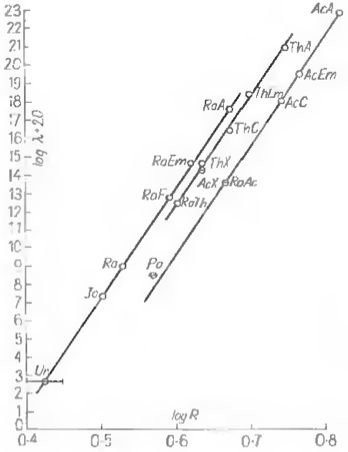
\includegraphics[width=(\textwidth-18mm),height=(\textheight-11mm),keepaspectratio]{lamalfvsR}
\caption{Probability of decay vs range}
\end{figure}

Usando l'espressione approssimata
\begin{align*}
G\approx\frac{\pi zZe^2}{\hbar v}-\frac{2e}{\hbar}\sqrt{2zZmR}&\intertext{per}\\
x=u=(\frac{E}{B})_{\text{Segre}}=(\frac{Q}{B})_{\text{quad}}\ll1
\end{align*}
scrivo
\begin{equation*}
\ln{\lambda}=-\frac{\sqrt{2mB}}{\hbar}a[\pi\sqrt{\frac{B}{Q}}-4]+\ln{v_0}{a}
\end{equation*}

$B=V(r=a)$ \'e funzione di $a$ che va come $A^{\frac{1}{3}}$, ci aspettiamo che per una serie di isotopi $\ln{\lambda}$ sia una funzione lineare di $Q^{-\frac{1}{2}}$.

Original figure of Geiger and Nuttal showing the connection between range (percorso particella alpha) and decay constant in \Ra-particle decay.


Riprendo $P=\exp{-2G}$, dove $G$ \'e il fattore di Gamow, e analizzo l'integrale $\frac{\sqrt{2m}}{\hbar}\int_a^b\sqrt{V(r)-q}dr$ con i vincoli imposti dal problema:

\lbt{B=\alpha_{FS}\hbar c\frac{Z_{\alpha}Z_Y}{a}}{b=\alpha_{FS}\hbar c\frac{Z_{\alpha}Z_Y}{Q}}.

\begin{align*}
\sqrt{V(r)-Q}=\sqrt{Q}\sqrt{\alpha_{FS}\hbar c\frac{Z_{\alpha}Z_Y}{Q}\frac{1}{r}-1}=\sqrt{Q}\sqrt{\frac{b}{r}-1}
\end{align*}
quindi pongo $x=\frac{r}{b}$ e ho $\sqrt{V(r)-Q}=\sqrt{Q}\sqrt{\frac{1}{x}-1}$ e infine
\begin{equation*}
G=\frac{\sqrt{2mQ}}{\hbar}b\int_{x_0=\frac{a}{b}}^1\sqrt{\frac{1}{x}-1}dx
\end{equation*}

\subsection{Funzione gamma: encore}

\begin{align*}
G=\frac{2z_{\alpha}Z_Ye^2}{\hbar v}\gamma(x)=2z_{\alpha}Z_Y\alpha_{SF}\frac{c}{v}\gamma(x)&\intertext{ho definito:}\\
\gamma(x)=\arccos{x^{\frac{1}{2}}}-x^{\frac{1}{2}}(1-x)^{\frac{1}{2}}\\
x=\frac{a}{b}=\frac{Q}{B}\\
v=\sqrt{\frac{2Q}{m}}
\end{align*}

Per $x=\frac{Q}{B}\ll1$ (grossolanamente)
\begin{align*}
\gamma(x)\to(\frac{1}{2})\pi-2x^{\frac{1}{2}}\\
G\approx\frac{\pi z_{\alpha}Z_Ye^2}{\hbar v}-\frac{2e}{\hbar}(2z_{\alpha}Z_Yma)^{\frac{1}{2}}
\end{align*}

\subsection{Formula di Gamow}
Per $u_{min}=x_0=\frac{a}{b}\ll1 (a\ll b)$ approssimo:

$F(x_0)\approx\frac{\pi}{2}-2\sqrt{x_0}=\frac{\pi}{2}-2\sqrt{\frac{Q}{B}}$.

Quindi scrivo il fattore di Gamow:

$G=\frac{\sqrt{2mQ}}{\hbar}b[\frac{\pi}{2}-2\sqrt{\frac{Q}{B}}]$.

La costante di decadimento \'e $\lambda=\frac{1}{\tau}=f*P=$:

prendo il logaritmo da ambo le parti e, trascurando termini contenenti potenze positive di $\frac{E}{B}$, ho l'equazione di Gamow 

\begin{align*}
&\ln{\tau}=\ln{(\frac{a}{c}\sqrt{\frac{m_{\alpha}c^2}{2(Q+V_0)}})}\\
&+2\alpha_{FS}Z_{\alpha}Z_Y\sqrt{2m_{\alpha}c^2}[\frac{\pi}{2\sqrt{Q}}-\frac{2}{\sqrt{B}}]&\intertext{dove \'e esplicitata la dipendenza da Q}\\
&\log{\lambda}=\frac{-\sqrt{2mB}}{\hbar}a[\pi\sqrt{\frac{B}{Q}}-4]+\log{\frac{v}{a}}&\intertext{Dato che $B=\frac{e^2z_{\alpha}Z_Y}{a}\propto\frac{e^2z_{\alpha}Z_Y}{A^{\frac{1}{3}}}$, per una serie di isotopi ci aspettiamo dipendenza lineare di $\log{\lambda}$ da $\sqrt{Q}$}
\end{align*}

Numericamente abbiamo la formula (scritta da Taagepera e Nurmia)
\begin{equation*}
\log{\thalf}=1.61(ZQ^{-\frac{1}{2}}-Z^{\frac{2}{3}})-28.9
\end{equation*}
where $\thalf$ is the half-life in years, Q is in MeV and Z refers to daughter nuclei.

From experimental known decay constant and energies of \Ra-particles one  finds that nuclear radius value calculated from ground transition of even-even nuclei follow the law:

$R=a=1.5*10^{-13}A^{-\frac{1}{3}}cm$.

\subsection{Emissione di nuclei pi\'u pesanti di \Ra}
Detta $w_Y$ la probabilit\'a che la particella emessa si sia formata per fluttuazioni casuali all'interno del nucleo ($w_Y\ll w_{\alpha}$).
Esempio: Decadimento $^{220}Th$.

\begin{itemize*}
\item \Ra-emission: $^{220}_{90}Th\rightarrow^{216}_{88}Ra+\alpha$\\
\lbt{Q=8.95 MeV}{\tau=9.7*10^{-9}s}
\item $^{12}_6C$-emission: $^{220}_{90}Th\rightarrow^{208}_{84}Po+^{12}_6C$\\
\lbt{Q=32.14}{\tau=3.3*10^6}
\end{itemize*}
L'altezza della barriera Coulombiana va come $zZ$:

\lbt{B_{\alpha}=V_{\alpha}(r=a)\propto z_{\alpha}Z_Y=176}{B_C=V_C(r=a)\approx z_CZ_Y=504}, questo favorisce l'emissione di \Ra.

\chapter{Struttura fine degli spettri alfa}

\section{Leggi di conservazione: regole di selezione}

\begin{itemize*}
\item Conservazione momento angolare\\
$\vec{I_i}=\vec{l}_{\alpha}+\vec{I}_f$ cio\'e $l_{\alpha}=I_i+I_f,\ldots,|I_i-I_f|$.
\item Conservazione della parit\'a\\
$\Pi_i=\Pi_f(-1)^{l_{\alpha}}$
\end{itemize*}

\section{Fattori di ritardo del decadimento}
I decadimenti \Ra  negli stati eccitati sono meno probabili:

Il decadimento dei nuclei pari-pari tra livello fondamentale e livello fondamentale mostrano la costante di decadimento pi\'u alta, other transitons are hindered in varying degrees. 
\begin{itemize*}
\item $Q^*=Q^0-E^*$ quindi $Q^*<Q^0$: considerando i canali di decadimento verso nuclei eccitati si ha una vita media maggiore quindi minore probabilit\'a di decadimento
\item Per $l\neq0$ il termine repulsivo $\frac{l(l+1)\hbar^2}{2mr^2}$ rende la barriera di potenziale pi\'u spessa.
\item Departure of nucleus from spherical form may also produce hindrance.
\end{itemize*}
 
\subsection{Eccitazioni rotazionali dello stato fondamentale}
Oltre la banda dello stato fondamentale la probabilit\'a di decadimento diventa molto piccola: molte eccitazioni oltre la banda  fondamentale sono vibrazioni disaccoppiamento di 2 nucleoni e perci\'o la funzione d'onda iniziale e finale saranno diverse. 

 \begin{figure}[!ht]
\centering
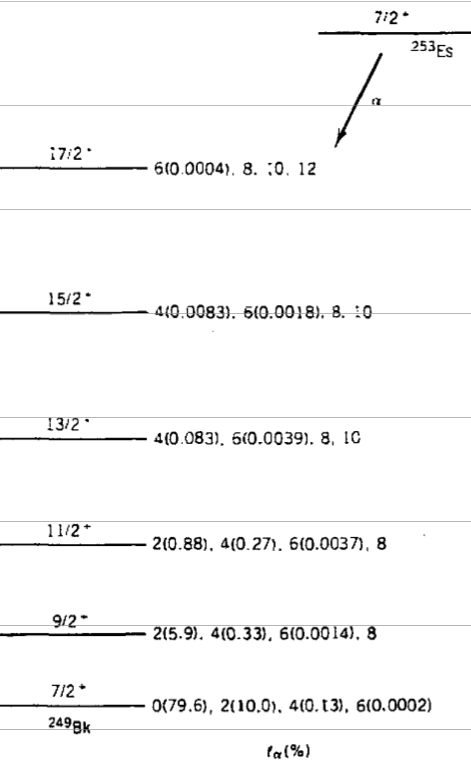
\includegraphics[width=(0.5\textwidth),height=(\textheight),keepaspectratio]{adecaydes}
\caption{$\alpha$ decay to different excited states.}
\end{figure}

To determine $l_{\alpha}$ we have to know the spatial distribution of \Ra-particle: per esempio se la distribuzione spaziale \'e proporzionale a $Y_3(\theta,\phi)$ \'e $l_{\alpha}=3$. Per fare questo tipo di misure devo allineare gli spins dei nuclei radiattivi, per esempio allineando il momento di dipolo magnetico o quadripolo elettrico in un campo magnetico o in presenza di un gradiente di campo elettrico, come quelli cristallini, temperatures below $0.01K$ are required.Intensity of varous \Ra-decay angular momentum component: neither the initial nor the final states have spin 0

\section{\Ra-ray spectroscopy}

\subsection{Decadimento del Plutonio-238}
Decadimento \Ra: $^{238}Pu\rightarrow^{234}U+\alpha$: bande rotazionali.

\subsection{Population of $^{247}Cf$ excited level via \Ra-decay of $^{251}Fm$}

There are 13 groups of \Ra particles, each group presumably represents the decay to a different excited state of $^{247}Cf$, to find the decay energies we use the relation $T_{\alpha}=Q(1-\frac{4}{A})$. In even-even decay would be a good assumption that the highest energy \Ra decay populate the ground state of child nucleus because the $0^+\rightarrow0^+$ alpha decays are very strong and not inhibited by any differences between the wavefunction of initial and final nuclear states; in the odd-A case initial and final ground state may have different character. Let's guess that the first three states are those associated with the energies $0$, $55.0 KeV$ and $122.1 KeV$ and that states form a rotational band; using the shell model we say that an odd-A (deformed) nucleus have angular momentum $I=\Omega,\Omega-1,\Omega-2,\ldots$ where $\Omega$ is the component of the angular momentum of the odd particle along symmetry axis: 

the energy differences between the ground state and the first excited state, and others ,
being $E=\frac{\hbar^2}{2\mathcal{I}}I(I+1)$ the energy of rotational states, are
\begin{align*}
\Delta E_{21}=E_2-E_1&=\frac{\hbar^2}{2\mathcal{I}}[(\Omega+1)(\Omega+2)-\Omega(\Omega+1)]=\frac{\hbar^2}{2\mathcal{I}}2(\Omega+1)\\
\Delta E_{31}=E_3-E_1&=\frac{\hbar^2}{2\mathcal{I}}2(2\Omega+3)
\end{align*}
Comparison with experimental values
\begin{align*}
\Delta E_{21}=55.0 KeV\\
\Delta E_{31}=122.1 KeV
\end{align*}

we conclude that 
\begin{align*}
\Omega=3.5=\frac{7}{2}\\
\frac{\hbar^2}{2\mathcal{I}}=6.11 KeV
\end{align*}

\section{Tecniche sperimentali}
\subsection{Ostacoli rilevamento \Ra-decay}
The disintegration constant must also not be too small or else \Ra emission will occur so rarely that it may not be detected: with present (late '80) technique half-life must be less than about $10^{16} y$; also \Rb-decay if it has a much higher partial disintegration constant can mask the \Ra-decay. Most nuclei with $A>190$ (and many with $150<A<190$) are energetically unstable against \Ra-emission but only in one-half of them is easily observable.

\index{la parte finale dell'alpha decay \'e superflua???????}

\chapter{Fusione}

\sectio{Fenomenologia della fusione}

\subsection{Coulomb barrier}
\begin{align*}
&V=\frac{e^2Z_aZ_X}{R}=1.44\frac{Z_aZ_X}{R(fm)}\\
&B_{aX}=V_{aX}(r=R_a+R_X)=\alpha_{SF}\hbar c\frac{Z_aZ_X}{R_a+R_X}
\end{align*}

\begin{align*}
B_{PP}\approx 0.9 MeV\\
B_{DT}\approx 0.4 MeV
\end{align*}



\section{Fusion between 2 Ne nuclei.}

\subsection{Heavy Ion Collider.}

Accelerating $^{20}Ne$ to $21.2 MeV$ against $^{20}Ne$ target.

\subsection{Thermal energy to overcome Coulomb B.}
For $^{20}Ne$ $\frac{1}{2}*21.2 MeV=\frac{3}{2}KT$ quindi $T=10^{11}K$.

\section{Alcune reazioni di fusione}

\subsection{DD fusion}
\begin{align*}
^2H+^2H\to^4He+\Pphoton\quad(Q=23.8\,MeV)&\intertext{dato che $Q>S_{\Pproton},\,S_{\Pneutron}$ i seguenti processi son pi\'u probabili}\\
^2H+^2H\to^3He+\Pneutron\quad(Q=3.3\,MeV)\\
^2H+^2H\to^3He+\Pproton\quad(Q=4.0\,MeV)
\end{align*}

\section{Energetica della fusione.}

\subsection{Q di fusione: energy release.}

\begin{equation*}
Q=[(m_a+m_X)-(m_b+m_Y)]c^2
\end{equation*}

\subsection{Distribuzione energia cinetica dei prodotti di fusione.}

For most applications of fusion I can neglect the initial motion of reagents

\begin{align*}
&\frac{1}{2}m_bv_b^2+\frac{1}{2}m_Yv_Y^2=Q & \intertext{Energy eq}\\
&m_bv_b=m_Yv_Y & \intertext{Conservazione del momento}
\end{align*}

e ricavo

\begin{equation*}
\frac{T_b}{T_Y}=\frac{m_Y}{m_b}
\end{equation*}

\subsection{Binding energy.}
 Dal grafico della BE/A in funzione di A vedo che la fusione \'e esoenergetica ($Q>0$) fino ad $A=56$ (produco elementi pi\'u legati fino al $^{56}Fe$).


\section{Esempi di Fusion Reaction.}

\subsection{DD reactions.}
$B_{DD}=360KeV$

\begin{align*}
^2H+^2H\to ^4He+\gamma (Q=23.8Mev)\\
^2H+^2H\to ^3He+n (Q=3.3 MeV)\\
^2H+^2H\to ^3H+p (Q=4.0 MeV) \intertext{Lighter products have $75\%$ of Q}
\end{align*}

\subsection{DT reactions}

\begin{align*}
^2H+^3H\to ^4He+n (Q=17.6 Mev)& \intertext{Neutron monoenergetic ($80\%$ of Q)}\\
T_n=\frac{Q}{1+\frac{m_n}{m_{He}}}\approx14.1 MeV &
\end{align*}


\chapter{Reaction Rate di fusione.}

\subsection{Sezione d'urto di Rutherford}

\begin{align*}
\frac{d\sigma}{d\Omega} &=\frac{\text{Events into solid angle $d\Omega$ at $(\theta,\phi)$/(unit time)}}{d\Omega*(\text{Incident particles})*(\text{Target nuclei}/cm^2)}\\
\frac{d\sigma}{d\Omega} &=(\frac{\alpha}{2m{v_{\infty}}^2})^2\frac{1}{\sin^4{\frac{\theta}{2}}}\\
\frac{d\sigma}{d\Omega} &=(\frac{(ze)(Ze)}{4k})^2(\frac{1}{4\pi\epsilon_0})^2\frac{1}{\sin^4{\frac{\theta}{2}}}
\end{align*}

per un sistema di riferimento in cui il centro di massa delle particelle \'e a riposo.

\subsection{Sezione d'urto non risonante}
Particelle interagenti ad energie "termiche" \'e probabile che non siano in zone di risonanza per la sezione d'urto di fusione.

La sezione d'urto \'e proporzionale a:
\begin{enumerate*}
\item Fattore $k^{-2}$
\item Partial reaction probability.

Per particelle cariche include un fattore che tiene conto della probabilit\'a di attraversamento della barriera di potenziale 

\begin{align*}
\exp{-2G}=\exp{-\frac{2\pi Z_aZ_Xe^2}{\hbar v}}
\end{align*}

\end{enumerate*}

cio\'e la relazione $\sigma_{Fus}\propto\frac{1}{v^2}\exp{-2G}$ include tutta la dipendenza energetica.

Il fattore di proporzionalit\'a coinvolge elementi di matrice nucleare e fattori statistici dipendenti dagli spin.

$\sigma_{FUS}=\sigma(aX\to bY)*P$:

P \'e la probabilit\'a di attraversamento della barriera Coulombiana.

$\sigma(aX\to bY)$ dipende da elementi di matrice nucleare e fattori statistici relativi agli spin delle particelle.

Per includere la debole dipendenza da E per fusione non risonante scrivo:

$\sigma_{FUS}=\frac{S(E)}{E}\exp{-2G}$:

$S(E)$ \'e chiamato fattore astrofisico.

La dipendenza $\propto\frac{1}{E}$ \'e un fattore geometrico.

\subsection{Probabilit\'a attraversamento barriera Coulombiana}
La probabilit\'a di attraversare una barriera infinitesima $[r,r+\,dr]$ 
\begin{align*}
dP=\exp{-2\,dr\sqrt{\frac{2m}{\hbar^2}}\sqrt{V(r)-E}}&\intertext{che per barriera finita}\\
P=\exp{-2G}
\end{align*}

Energia di Gamow: $E_G$.

\begin{align*}
P\propto\exp{-\sqrt{\frac{E_G}{E}}}&\intertext{Definita l'energia}\\
E_G=2mc^2(\pi \alpha_{SF}Z_aZ_X)^2
\end{align*}

\subsection{"Gamow Factor": alpha decay vs fusion}

Avendo in mente la probabilit\'a di attraversamento di una barriera Coulombiana calcolata nella teoria del alpha decay.

\begin{align*}
G=\sqrt{\frac{2m}{\hbar^2}}\int_a^b\sqrt{V(r)-E}\,dr & \intertext{con $x=\frac{Q}{B}$}\\
&\intertext{nel caso della fusione sostutuisco Q con E=center of mass energy of reacting particles}
E\approx KeV\ll B&\intertext{approssimo}\\
G\approx\frac{e^2}{4\pi\epsilon_0}\frac{\pi Z_aZ_X}{\hbar v}=\pi\alpha_{SF}\frac{Z_AZ_X}{v/c}
\end{align*}

Riscrivo G: per praticit\'a raggruppo le costanti del fattore di Gamow in $\beta$.

\begin{equation*}
G=\beta\frac{1}{\sqrt{E}}=\frac{\pi}{2}\alpha_{SF}\sqrt{2mc^2}Z_aZ_X\frac{1}{\sqrt{E}}=\pi\alpha_{SF}\frac{Z_AZ_X}{v/c}
\end{equation*}

\section{Picco di Gamow}

\subsection{Distro di MB}
\begin{align*}
F_{MB}(v)=4\pi v^2(\frac{m}{2\pi k_B T})^{\frac{3}{2}}\exp{-\frac{mv^2}{2K_BT}}
\end{align*}

\subsection{Reaction Rate: costante di decadimento}
\begin{equation*}
R(aX\to bY)=\frac{\# \text{reazioni}}{\text{Tempo}*\text{Volume}}=\sigma(aX\to bY)n_X\Phi_a
\end{equation*}

definito il flusso delle particelle a 
\begin{equation*}
\Phi_a=\frac{N_a}{\text{Superficie}*\text{Tempo}}=\frac{n_aV}{S*T}=n_av
\end{equation*}
quind
\begin{align*}
R&=n_an_X\exv{\sigma(v_{\text{rel}}) v_{\text{rel}}}\\
&=n_an_X\lambda&\intertext{definito il reaction rate per coppia di particelle ($n_a=1/cm^3$)}\\
\lambda=\exv{\sigma_Fv}\\
R=\frac{1}{2}n_X^2\exv{\sigma v}& \intertext{per particelle identiche.}
\end{align*}

La densit\'a di potenza prodotta in una reazione binaria, detto $W_{aX}$ l'energia liberata in una singola reazione, \'e
\begin{equation*}
P_{aX}=n_an_X\exv{\sigma v}W_{aX}
\end{equation*}

\subsection{Massimo di $F_{MB}\sigma v$}

\begin{align*}
\exv{\sigma v}\propto\intzi\frac{1}{v}\exp{-2G}\exp{-\frac{mv^2}{2kT}}v^2\,dv\\
\exv{\sigma v}\propto\intzi\exp{-2G}\exp{-\frac{E}{kT}}\,dE
\end{align*}

\begin{align*}
\exv{\sigma_Fv}&=\intzi\sigma_FvF^{MB}(v)\,dv\\
&=\sqrt{\frac{8}{\pi m}}(K_BT)^{-\frac{3}{2}}\intzi S(E)\exp{-\frac{E}{KT}-\frac{\beta}{\sqrt{E}}}\\
&\approx\sqrt{\frac{8}{\pi m}}(K_BT)^{-\frac{3}{2}}S_0\intzi \exp{-\frac{E}{KT}-\frac{\beta}{\sqrt{E}}}&\intertext{tutta ci\'o che non sappiamo sono i fattori astrofisici estrapolati a basse energia.}
\end{align*}
\index{Fattore astrofisico: energia zero.}

L'integrando \'e fortemente piccato quindi le particelle che danno maggiormente luogo a fusione (a parit\'a di condizioni) son quelle con picco pi\'u alto
\begin{equation*}
\frac{d}{dE}(\frac{E}{KT}+bE^{-\frac{1}{2}})_{E=E_0}=\frac{1}{KT}-\frac{1}{2}b(\frac{1}{E_0})^{\frac{3}{2}}
\end{equation*}
ovvero

\begin{align*}
&E_0=(\frac{bKT}{2})^{\frac{2}{3}}&\intertext{con}\\
A=\frac{A_1A_2}{A_1+A_2}=\frac{m}{m(u)}\\
&E_0=1.22(Z_a^2Z_X^2AT_6^2)^{\frac{1}{3}} (keV)&\intertext{Most effective energy for thermonuclear reactions}
\end{align*}

\index{Energia del picco di Gamow}

\subsection{Variazione di concentrazione dei reagenti}

\begin{align*}
&R=n_an_X\exv{\sigma v}&\intertext{Reaction rate medio}\\
&\lambda_a(X)=\frac{1}{\tau_a(X)}=\frac{\text{Probabilit\'a di fusione a-X}}{\text{Tempo}*\text{Nucleo X}}
\end{align*}

quindi
\begin{align*}
\frac{\partial n_X(t)}{\partial t}|_a&=-\lambda_a(X)n_X(t)=-\frac{n_X(t)}{\tau_a(X)}\\
&=-R_{aX}=-n_an_X\exv{\sigma_{aX}v}&\intertext{la vita media per la reazione $a+X$ \'e}\\
\tau_a(X)=\frac{1}{n_a\exv{\sigma_{aX}v}}
\end{align*}

\section{Risonanze nella fusione}

\subsection{Low energy capture reaction: compound nucleus}

La sezione d'urto di fusione di alcune reazioni ha dei picchi di risonanza:
\begin{equation*}
^1H+^{12}C\to^{13}N+\gamma\quad E\approx0.5 MeV
\end{equation*}

\begin{equation*}
\sigma_{ris}=\frac{\pi}{k^2}\frac{2J+1}{(2J_a+1)(2J_X+1)}\frac{\Gamma_{aX}\Gamma_{bY}}{(E-E_R)^2+\frac{\Gamma^2}{4}}
\end{equation*}

\section{Meccanismo di fusione nel stelle}

\subsection{PP cycle}

Nell'interno stellare l'idrogeno \'e ionizzato quindi nel caso di emissione di positroni nel Q-valore \'e compreso un contributo per l'annichilamento \Pelectron\APelectron.

\subsection{Bottle-neck}

\begin{align*}
&^1H+^1H\to^2H+\APelectron+\Pnue (Q=1.44 MeV)&\intertext{Il neutrino ha spettro continuo con endpoint}\\
&E(\nu)=0.42 MeV
\end{align*}

Reazione lenta:

\begin{align*}
&\sigma\approx 10^{-33}b (KeV)\\
&\approx 10^{-23} b (MeV)\\
&R=\frac{1}{2}n_P^2\exv{\sigma v}\approx5*10^{-18} \text{reazioni}/\text{P}/s\\
&\rhosunc=125gr/cm^3 \quad (7.5*10^{25}P/cm^3)\\
&\tsunc 15*10^6K\Rightarrow\exv{T_P}\approx1 KeV&
\intertext{per le regioni centrali del sole.}
\end{align*}

\subsection{Deuteron cooking up to Helium}

Il deutone viene trasformato rapidamente in isotopo di elio
\begin{equation*}
^2H+^1H\to ^3He+\gamma \quad (Q=5.49 MeV)
\end{equation*}

\subsection{Produzione di He4: ciclo PP1 (Sun:$69\%$).}
\begin{equation*}
^3He+^3He\to^4He+2^1H+\gamma\quad(Q=12.86 MeV)
\end{equation*}

\subsection{Bilancio energetico PP}
L'energia dei neutrini che escono dal core non scalda la fotosfera.
\begin{align*}
Q=26.7 MeV &\intertext{Atomi neutri e annichilamento \Pelectron\APelectron.}
\end{align*}

\subsection{Tempi medi di reazione nella catena PP.}
Per le condizioni presenti nel sole:

\begin{tabular}{c|c|}
\hline
Reazione & $t_r$ \\
\hline
$^1H+^1H\to^2H+\APelectron+\Pnue$ & $7*10^9\,yr$\\
$^2H+^1H\to ^3He+\gamma$ & $4 s$\\
$^3He+^3He\to^4He+2^1H$ & $4*10^5\,yr$\\
$^{12}C+^1H\to ^{13}N+\gamma$ & $10^6\, yr$\\
$^{13}N\to^{13}C+\APelectron+\Pnue$ & $10\,min$\\
$^{13}C+^1H\to ^{14}N+\gamma$ & $2*10^5\, yr$\\
$^{14}N+^1H\to ^{15}O+\gamma$ & $<3*10^7\, yr$\\
$^{15}O\to^{15}N+\APelectron+\Pnue$ & $2\,min$\\
$^{15}N+^1H\to ^{12}C+^4He$ & $10^4\, yr$\\
\hline
\end{tabular}

\section{Altre diramazioni della catena \Pproton\Pproton dopo produzione He3.}

\subsection{Ciclo HeP (Sun: $0.0001\%$).}
\begin{align*}
^3He+^1H\to^4He+\APelectron+\Pnue \quad (Q=19.28 MeV)\\
E_{\nu}^{max}=Q-m_ec^2=18.77 MeV
\end{align*}

\subsection{Produzione Be7 (Sun: $31\%$).}
\begin{equation*}
^3He+^4He\to^7_4Be+\gamma
\end{equation*}
da cui seguono 2 diramazioni:

\subsection{Ciclo PP2 (Sun: $99.7\%$).}
\begin{align*}
^7_4Be+\Pelectron\to^7_3Li+\Pnue&\intertext{CE: decadimento a 2 corpi: neutrino monoenergetico}\\
E(\nu)\approx0.862 MeV\\
^7_3Li+^1H\to2^4He
\end{align*}

\subsection{Ciclo PP3 (Sun: $0.3\%$).}
\begin{align*}
^7_4Be+^1H\to^8_5B+\gamma\\
^8_5B\to^8_4Be+\APelectron+\Pnue&\intertext{Spettro energetico del neutrino continuo con endpoint}\\
E(\nu)=14 MeV\\
^8_4Be\to2^4He
\end{align*}

\subsection{Energia irradiata in neutrini}
\begin{align*}
Q_{eff}&=Q-\exv{E_{\nu}}(MeV)\quad&\text{Perdita in neutrini}&\intertext{PP1}\\
&=26.2 &2\%&\intertext{PP2}\\
&=25.66  & 4\%&\intertext{PP3}\\
&=19.17  & 28\%
\end{align*}


\section{Ciclo CNO}
Procede con maggiore velocit\'a perch\'e non \'e presente il bottleneck $H+H\to D$ ma la barriera coulombiana per la fusione dei nuclei \'e 6-7 volte pi\'u elevata: efficiente ad alte temperature.

\begin{figure}[!ht]
\centering
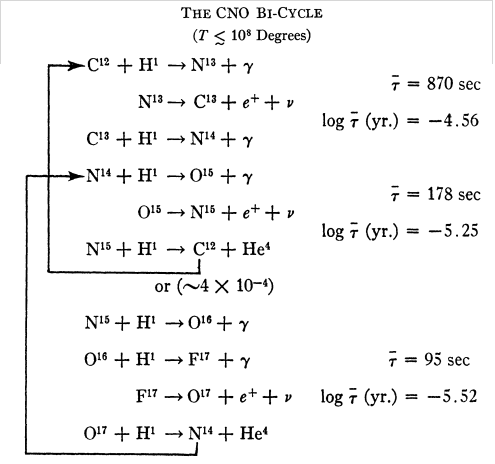
\includegraphics[width=(\textwidth),height=(\textheight-11mm),keepaspectratio]{cnobi}
\caption{Bi-ciclo CNO.}
\end{figure}

\begin{align*}
^{12}_6C+^1H\to^{13}_7N+\gamma\\
^{13}N\to ^{13}_6C+\APelectron+\Pnu\\
^{13}C+^1H\to ^{14}_7N+\gamma\\
^{14}_7N+^1H\to ^{15}_8O+\gamma\\
^{15}_8O\to ^{15}_7N+\APelectron+\gamma\\
^{15}_7N+^1H\to ^{12}_6C+^4_2He
\end{align*}

Processo efficace:

$4^1H\to ^4He+2\APelectron+2\Pnue$ uguale alla catena PP, stesso Q-valore.

\section{Evoluzione stellare}

\subsection{Modello standard del sole}

\begin{align*}
&\msun=2*10^{33}gr\\
&\text{Age}=4.55*10^9\,yr\\
&\rsun=7*10^5 Km\\
&\tsunc=1.57*10^7 K\\
&\tsuns=6*10^3 K\\
&\rhosunc=130gr/cm^3\\
&\lsun=3.8*10^{26}W=3.8*10^{33}erg/s\\
&\Phi_{\nu}(\Pproton\Pproton)=6.0*10^{10}cm^{-2}s^{-1}\\
&\Phi_{\nu}(^8B\to^8Be^*+\APelectron+\Pnue)=6.0*10^6cm^{-2}s^{-1}\\
&X=74\%,\,Y=23,\,Z=3&\intertext{$\uparrow$ Attuale}\\
&X=75\%,\,Y=22,\,Z=3&\intertext{$\uparrow$ Composizione iniziale}\\
\end{align*}

\subsection{Equilibrio idrostatico.}
\begin{align*}
dS\,(P(r)-P(r+\,dr)-F_g(r))=0\\
F_g(r)=G\frac{m(r)\rho(r)\,dV}{r^2}&\intertext{se ho simmetria sferica}\\
\frac{dm}{dr}=4\pi\rho(r)r^2
\end{align*}

Posso trascurare la BE gravitazionale?
\begin{align*}
B_{\odot}=N_Pm_p-\msun=-E_G=\frac{3}{5G\frac{\msun^2}{\rsun}}\approx10^{-6}\msun c^2
\end{align*}

\subsection{Equazione di stato.}

\begin{align*}
&P=P(\rho,T,X,Y,Z)=P_{Gas}+P_{Rad}&\intertext{Gas ideale}\\
&P_{Gas}=K\rho T\\
&P_{Rad}=\frac{1}{3}aT^4
\end{align*}

\subsection{Produzione di energia}
\begin{align*}
\epsilon=\frac{\text{Energia prodotta}}{\text{Massa}*\text{Tempo}}&\intertext{L'energia prodotta per fusione}\\
\epsilon=\epsilon_F(\exv{\sigma v},\rho,T,X,Y,Z)&\intertext{\'e legata alla luminosita tramite}\\
\frac{d\lu}{dr}=\epsilon_F(r)4\pi r^2
\end{align*}

\subsection{Reaction Rate}
La radiazione che raggiunge la terra ha un flusso di $1.4*10^3 W/m^2$ quindi la potenza irraggiata \'e $4*10^{26} W$: dato che ogni reazione di fusione libera 25 MeV sono necessarie $10^{38} \text{Fusioni}/sec$ (4 $^1H$ per fusione).

\begin{equation*}
N_{Reaz}=\frac{\exv{R_{PP}}}{n_P}N_p(core)
\end{equation*}

\subsection{Flusso neutrini}
\begin{equation*}
\Phi_{\nu}=\frac{\dot{N_{\nu}}}{4\pi d^2}=7*10^{10}\frac{\Pnu}{s*cm^2}
\end{equation*}

\section{Fasi finali dell'evoluzione stellare.}

\subsection{Teorema del viriale}
Relazione tra l'energia cinetica media e l'energia potenziale di un sistema in equlibrio stabile o quasi-stabile.

\begin{align*}
&G=\sum_i\scap{p_i}{r_i}=\frac{1}{2}(\sum_im_ir_i^2)^2=\frac{1}{2}\frac{dI}{dt}&\intertext{I momento d'inerzia}\\
&\frac{dG}{dt}=\sum_i\scap{\dot{r_i}}{p_i}+\sum_i\scap{r_i}{\dot{p_i}}=2T+\sum_i\scap{r_i}{f_i}&\intertext{l'ultimo termi del membro di destra \'e il  viriale di Clausius}\\
&\intertext{Assumendo che la forza tra le particelle segua una legge di potenza della distanza con esponente n(del potenziale) e sia derivabile da un potenziale}\\
&\frac{dG}{dt}=2T-n\mathcal{U}&\intertext{dove U \'e l'energia potenziale totale del sistema}\\
&\frac{dG}{dt}=\frac{1}{2}\frac{d^2I}{dt^2}=2T+\Omega&\intertext{per il potenziale gravitazionale n=-1}\\
&2\overline{T}+\overline{\Omega}=0&\intertext{se il sistema \'e periodico la media del lato sinistro su un periodo dell'equazione sopra \'e nullo}
\end{align*}

\subsection{Fasi di contrazioni ed espansioni successive.}

Terminato l'idrogeno il core di elio si contrae non essendoci pi\'u fonti di energia fino a che si raggiungono T sufficienti per la fusione di dell'elio.

Detti m massa del core e r suo raggio
\begin{align*}
E_G=-G\frac{m^2}{r}&\intertext{quindi in fase di contrazione}\\
\Delta E_G=\frac{Gm}{r^2}\Delta r<0&\intertext{da cui risulta aumento di energia cinetica}\\
\Delta E=-\frac{1}{2}\Delta U_G>0
\end{align*}

\subsection{fase di fusione dell'elio ($T\approx10^8K$).}

Fusione di elio-4 in carbonio-12
\begin{align*}
^4He+^4He\to ^8_4Be\quad(\tau\approx10^{-16}s)\\
^8Be+^4He\to^{12}C+\gamma&\intertext{al crescere di T}\\
^{12}C+^4He\to ^{16}O+\gamma\\
^{16}O+^4He\to^{20}Ne+\gamma
\end{align*}

\subsection{Fase di fusione del carbonio-12.}
\begin{align*}
^{12}C+^{12}C&\to ^{16}O+2^4He\\
&\to ^{20}Ne+^4He\\
&\to ^{23}Na+\Pproton\\
&\to^{24}Mg+\gamma
\end{align*}

\subsection{Fase fusione Ossigeno.}
\begin{align*}
^{16}O+^{16}O&\to ^{28}_{14}Si+^4He\\
&\to^{31}_{15}P+\Pproton\\
&\to ^{32}S+\gamma
\end{align*}

e cos\'i via fino al $^{56}Fe$ per le stelle pi\'u massicce.

\subsection{Destino finale della stella}

\begin{itemize*}
\item $M<8\msun$: Nane bianche ($R\approx R_T$).
La pressione di degenerazione degli elettroni blocca il collasso.

\item $8\msun<M<25\msun$: stella di neutroni.
La nucleosintesi raggiunge il $^{56}Fe$  poi hanno luogo fenomeni di cattura elettronica (neutronizzazione della materia): sintesi elementi pi\'u pesanti.

\item $M>25\msun$: buco nero.

\end{itemize*}


\section{Nane bianche}

\subsection{Grandezze caratteristiche}

\begin{itemize*}
\item $M\approx\msun$
\item $\rho_c\approx10^6gr/cm^3\approx10^4\rhosunc$.
\begin{align*}
n_e=\exv{Z}n_I\\
\rho&=\exv{m_I}n_I+m_en_e\\
&\approx\exv{M_{atom}}n_I=\exv{A}m_Hn_I
\end{align*}

\item Raggio di Schwarzschild.

\begin{equation*}
\frac{R_G}{R}\approx100(\frac{R_G}{R})_{\odot}\approx4*10^{-6}
\end{equation*}
ho definito il raggio di Schwarzchild come $R_G=\frac{2GM}{c^2}$.
\item Velocit\'a di fuga.

\begin{equation*}
v_f=\sqrt{\frac{2GM}{R}}\approx0.02 c
\end{equation*}

\item Pressione.

\begin{equation*}
P=P_I+P_{el}\approx P_{el}
\end{equation*}
\end{itemize*}

\subsection{How far inward before degeneracy set in?}
Condizione necsuff perch\'e si abbia degenerazione \'e
\begin{align*}
\frac{4\pi^2}{(\theta mc^2)^2}\frac{x\sqrt{x^2+1}}{f(x)}\gg1&\intertext{ho definito}\\
x=\frac{h}{mc}(\frac{3n}{8\pi})^{\frac{1}{3}}\quad \theta=\frac{1}{KT}
\end{align*}
Per gli strati esterni vale $P\propto\rho T$ ($\approx0.23 \%$ della massa) 


\subsection{Equazione di stato gas perfetto}

\begin{align*}
n=\frac{N}{V}\\
\rho=\frac{M}{V}\\
m_0=\frac{M}{N}&\intertext{\'e il peso molecolare medio}\\
\end{align*}
ho l'equazione di stato
\begin{align*}
PV=nRT=NKT&\intertext{Riscrivo l'equazione di stato esprimendo la pressione in funzione della densit\'a, temperatura e composizione}\\
P=(\frac{N}{V})KT=nKT=\frac{\rho}{m_0}KT\\
P=\frac{1}{\mu}\frac{K_B}{m_P}\rho T&\intertext{definisco il peso molecolare in termini di proton mass}\\
\frac{1}{\mu}=2X+\frac{3}{4}Y+\frac{Z}{2}
\end{align*}
\index{Peso molecolare: particelle libere. ???}

Ricavo la relazione densit\'a di energia cinetica-pressione.

\begin{align*}
\epsilon=\frac{E}{V}=\frac{1}{V}\frac{3}{2}NK_BT&\intertext{Relazione tra pressione e concentrazione degli elettroni.}\\
P=\frac{2}{3}\epsilon
\end{align*}

\subsection{Pressione di radiazione}
For radiative equilibrium
\begin{equation*}
F_{RAD}=-\frac{d}{dr}(\frac{a}{3}T^4)=-\frac{dP_R}{dr}
\end{equation*}

\subsection{Gas di Fermi non relativistico}

\begin{itemize*}

\item Degenerazione.

\begin{equation*}
n_e\,d^3x\,d^3p\leq2\frac{d^3x\,d^3p}{h^3}
\end{equation*}

\item Densit\'a di stati.


\begin{align*}
dN=\frac{1}{8}4\pi n^2dn&\intertext{da cui ricavo la densit\'a imponendo le condizioni periodiche al bordo del volume $V=L^3$}\\
g(k)=\frac{dN(k)}{d^3k}=\frac{dN(k)}{4\pi k^2dk}=\frac{\nu V}{(2\pi)^3}
\end{align*}

\item Energia gas di Fermi completamente degenere: $T=0$.
\begin{equation*}
N=\int g(k)F(k)d^3k=\frac{\nu V}{(2\pi)^3}\int_0^{K_F}4\pi k^2\,dk=\frac{\nu V}{2\pi^2}\frac{k_F^3}{3}
\end{equation*}
da cui ricavo la densit\'a
\begin{equation*}
n=\frac{\nu}{6\pi^2}k_F^3
\end{equation*}

e adesso introduco la densit\'a di energia e ricavo la sua dipendenza da n
\begin{align*}
\epsilon=\frac{\hbar^2k^2}{2m_0}\quad(\epsilon_F=\frac{\hbar^2k_F^2}{2m_0})\\
E=\int\epsilon(k)F(k)g(k)d^3k=\frac{\nu V}{2\pi^2}\frac{\hbar^2}{2m_0}\frac{k_F^5}{5}\\
\frac{E}{N}=\frac{3}{5}\epsilon_F\\
\epsilon=\frac{E}{V}=\frac{E}{N}\frac{N}{V}=\frac{3}{5}\epsilon_Fn\propto n^{\frac{5}{3}}
\end{align*}
e per la pressione di un gas di Fermi di elettroni completamente degenere
\begin{align*}
P&=-\frac{\partial E}{\partial V}|_{S,N}=n^2\frac{\partial(\frac{E}{N})}{\partial n}|_{S,N}\propto n^{\frac{5}{3}}\\
P&=K_{NR}\rho^{\frac{5}{3}}
\end{align*}

\end{itemize*}



\subsection{Gas di Fermi relativistico}
\begin{itemize*}

\item Energia.

\begin{equation*}
\epsilon(k)=\sqrt{(\hbar ck)^2+(m_0c^2)^2}
\end{equation*}

\item Parametri adimensionali.

\begin{align*}
y=\frac{\hbar}{m_0c}k=\lambdabar k\\
\lambdabar k_F=x
\end{align*}

\item densit\'a di particelle.

\begin{equation*}
n=\frac{8\pi c^3m^3}{3h^3}x^3=5.87*10^{29}x^3
\end{equation*}

\item Energia cinetica.

\begin{equation*}
P\propto n^{\frac{4}{3}}
\end{equation*}

\end{itemize*}

\subsection{Relazione elettroni/Ioni}
\begin{equation*}
N_E=\frac{1}{\mu_E}\frac{\rho}{m_P}\quad\frac{1}{\mu_E}=X+\frac{1}{2}Y+\frac{1}{2}Z\approx\frac{1}{2}(1+X)
\end{equation*}

Condizioni per la degenerazione degli atomi: nuclei have on the average the same energy as electron, il momento \'e maggiore di un fattore radice quadrata del rapporto fra le masse per grado di libert\'a e quindi sono distribuiti nello spazio delle fasi su un volume $(2000)^{\frac{3}{2}}$ maggiore.
Per gli atomi possiamo usare
\begin{equation*}
P_A=\frac{1}{\mu_A}\frac{K}{m_P}\rho T\quad\frac{1}{\mu_A}=X+\frac{1}{4}Y
\end{equation*}

\subsection{Boundaries between D/ND and in latter R/NR}

Electron pressure for complete degeneracy
\begin{equation*}
P_E=\int_{|p|\leq p_0}\,d^3p\,p_xv_x\frac{2}{h^3}
\end{equation*}
e utilizzando l'opportuna relazione (R/NR) tra v e p trove la pressione nei due casi per gas di elettroni completamente degenere

\begin{itemize*}
\item Relativistico: $v=\frac{p}{m}$.
\begin{equation*}
P_E=\frac{2\pi c}{3h^3}p_0^4=K_2(\frac{\rho}{\mu_E})^{\frac{4}{3}}
\end{equation*}

\item Non relativistico $v_x=c\frac{p_x}{|p|}$.
\begin{equation*}
P_E=\frac{8\pi}{15mh^3}p_0^5=K_1(\frac{\rho}{\mu_E})^{\frac{5}{3}}
\end{equation*}

\end{itemize*}

\begin{itemize*}
\item Confine tra zona degenere e non degenere.

\begin{align*}
\frac{1}{\mu_E}\frac{K}{m_P}\rho T=K_1(\frac{\rho}{\mu_E})^{\frac{5}{3}}\\
\frac{1}{\mu_E}\rho=(\frac{KT}{m_PK_1})^{\frac{3}{2}}
\end{align*}
\item Confine tra zona degenere relativistica e non.

\begin{equation*}
\frac{1}{\mu_E}\rho=(\frac{K_2}{K_1})^3=1.916*10^6
\end{equation*}

\end{itemize*}

Il sole \'e descrivibile con equazioni non degeneri le nane bianche con equazioni degeneri.

\subsection{Mass/radius relation.}
L'equazioni di stato \'e indipendente da T
\begin{align*}
P=\frac{\pi m^4c^5}{3h^3}f(x)\\
\rho=\mu_E\frac{8\pi m_Pm^3c^3}{3h^3}x^3&\intertext{con}\\
x=\frac{p_0}{mc}\quad \mu_E=\frac{2}{1+X}
\end{align*}
Posso separare il problema idrostatico da quello termodinamico.

Equilibrio idrostatico:
\begin{align*}
\frac{dP}{dr}=-\rho\frac{GM_r}{r^2}\\
\frac{dM_r}{dr}=4\pi r^2\rho
\end{align*}
da integrare numericamente(Chandrasekhar).

Qualitativamente
\begin{itemize*}
\item The larger the mass of a white dwarf the smaller the radius.
\item Per nane bianche con circa massa solare il raggio \'e centinaia di volte pi\'u piccolo del sole.
\end{itemize*}

Limite superiore per la massa di una stella completamente degenere.

Quantit\'a che influenzano l'equilibrio idrostatico:
\begin{align*}
\rho\propto\frac{M}{R^3}&\intertext{questa sopra \'e la densit\'a, questa sotto l'attrazione gravitazionale}\\
\rho\frac{GM_r}{r^2}\propto\frac{M^2}{R^5}
\end{align*}

Per la pressione:
\begin{align*}
P\propto\rho^{\frac{5}{3}}\propto\frac{M^{\frac{5}{3}}}{R^5}&\intertext{per stelle meno massive ho la pressione NR (sopra), per stelle massive uso la formula R (sotto)}\\
P\propto\rho^{\frac{4}{3}}\propto\frac{M^{\frac{4}{3}}}{R^4}
\end{align*}

il cui gradiente genera una forza di pressione
\begin{align*}
F_P&\propto\frac{M^{\frac{5}{3}}}{R^6}\quad\text{NR-D}\\
&\frac{M^{\frac{4}{3}}}{R^5}\quad\text{R-D}
\end{align*}

Osservazioni:
\begin{itemize*}
\item In the relativistic case gravitational force and pressure force depend on the same power of radius.
\item In R-D the 2 forces depend on different power of mass.
\end{itemize*}

\subsection{Politrope}
Chiamo la funzione di sotto politropa di ordine n
\begin{equation*}
P=K\rho^{\gamma}=K\rho^{\frac{n+1}{n}}
\end{equation*}

\begin{itemize*}
\item Caso NR.
\begin{equation*}
P=K_{NR}\rho^{\frac{5}{3}}\quad N=\frac{3}{2}
\end{equation*}

\item Caso R.
\begin{equation*}
P=K_{UR}\rho^{\frac{4}{3}}\quad n=3
\end{equation*}
\end{itemize*}


Equazione di Lane-Emden:
Considero l'equilibrio idrostatico
\begin{align*}
\frac{dP}{dr}&=-G\frac{\rho(r)m(r)}{r^2}\\
\frac{dm}{dr}&=4\pi r^2\rho(r)&\intertext{con le condizioni al contorno:}\\
\rho(r=0)&=\rho_c\quad \rho=\frac{m_p}{Y_e}n_e=\mu_em_pn_e\quad\frac{1}{Y_e}=\frac{\exv{A}}{\exv{Z}}\\
\frac{d\rho}{dr}|_0&=0
\end{align*}
\index{Peso molecolare medio elettroni}

Riscrivo l'equazione dell'equilibrio idrostatico
\begin{equation*}
\frac{d}{dr}(\frac{r^2}{\rho(r)}\frac{dP}{dr})=-G\frac{dm(r)}{dr}=-G4\pi r^2\rho(r)
\end{equation*}
e ipotizzo 
\begin{align*}
\rho(\xi)=\rho_c\theta^n(\xi)&\intertext{e ho definito a con}\\
r=a\xi\quad a^2=\frac{(n+1)K}{4\pi G}\rho_c^{\frac{1-n}{n}}\\
P=K\rho^{\frac{n+1}{n}}=P_c\theta^{n+1}(\xi)
\end{align*}
per trovare la pressione devo risolvere l'equazione di Lane-Emden
\begin{align*}
\frac{1}{\xi^2}\frac{d}{d\xi}(\xi^2\frac{d\theta}{d\xi})=-\theta^n(\xi)&\intertext{con le condizioni al contorno}\\
\theta(\xi=0)=1\quad\frac{d\theta}{d\xi}|_{\xi=0}=0
\end{align*}

Raggio stellare: $\rho(r=R)=0$, primo zero della $\theta$.
\begin{equation*}
R=a\xi_1=B_n\rho_c^{\frac{1-n}{2n}}\quad\theta^n(\xi_1)=0
\end{equation*}

Massa stellare: $M=m(R)$.
\begin{equation*}
M=m(R)=m(a\xi_1)=\int_0^R\rho(r)4\pi r^2\,dr=A_n\rho_c^{\frac{3-n}{2n}}
\end{equation*}

Elimino la densit\'a centrale e ottendo una relazione tra massa e raggio
\begin{equation*}
M(n,R)=\frac{A_n}{B_n^{\frac{3-n}{1-n}}}R^{\frac{3-n}{1-n}}
\end{equation*}

\begin{itemize*}
\item Caso NR: $n=\frac{3}{2}$.
\begin{equation*}
M_{\frac{3}{2}}(R)\propto R^{-3}
\end{equation*}
\item Caso R: $n=3$.
\begin{equation*}
M_3(R)=const
\end{equation*}
\end{itemize*}

Trovo che esiste una massa limite per raggio tendente a zero e densit\'a infinita:
\begin{equation*}
M_{CSK}=M_3(R)=\frac{5.8\msun}{\mu_e^2}
\end{equation*}

\subsection{Interazione Ioni-elettroni}
Il contributo Coulombiano alla pressione diminuisce la massa limite:
\begin{equation*}
P_C\propto-e^2\exv{Z}^{\frac{2}{3}}n_e^{\frac{4}{3}}<0
\end{equation*}

%http://dujs.dartmouth.edu/wp-content/uploads/2008/04/09-whitedwarf.pdf
%http://upcommons.upc.edu/e-prints/bitstream/2117/18798/1/303_bravo.pdf
%http://www.astro.uvic.ca/~fherwig/TEACHING/ASTR501/StudentPresentations/EOS%20ASTR401%20MichaelP.pdf
%http://w.astro.berkeley.edu/~gmarcy/astro160/papers/physics_of_white_dwarfs.pdf
%

\chapter{Fissione}

\section{Fenomenologia. Criterio di stabilit\'a per deformazioni}

\subsection{Fissione spontanea vs fissione indotta}

\begin{itemize*}
\item Fissione spontanea.

I nuclei nella regione del $^{56}Fe$ hanno BE per nucleone maggiore fra tutti i nuclei quindi aumentando la massa la BE decresce: 

la BE($^{238}U$)/nucleone \'e $7.6 MeV$ da una fissione simmetrica si hanno 2 nuclei con BE($^{119}Pd$)/nucleone di circa $8.5 MeV$.

Energeticamente \'e possibile la fissione spontanea ma \'e un processo improbabile per la barriera di potenziale: ho un'elevata soglia di attivazione.


If Zero point energy of collective motion of nucleus produces a deformation we have a finite probability of fission by tunnel effect: 

vedremo in ~\ref{sec:deformednucleus} che una piccola deformazione modifica l'energia totale di

\begin{equation*}
\Delta E=B(0)-B(\epsilon)=\frac{\epsilon^2}{5}(2a_SA^{\frac{2}{3}}-a_CZ^2A^{-\frac{1}{3}})
\end{equation*}
se $\Delta E<0$ la deformazione \'e energeticamente favorita.

La barriera di fissione (vedi ~\ref{fig:fissionthreshold}) scompare  per $\frac{Z^2}{A}\geq\frac{2a_S}{a_C}\approx48$.

\item Fissione indotta.

Per nuclei pesanti ($Z\approx92$) la barriera di fissione \'e circa 6 MeV: questa energia pu\'o essere fornita tramite un flusso di neutroni lenti che induca processi di cattura neutronica che portano il nucleo in uno stato eccitato sopra la barriera di fissione.

I frammenti sono ricchi di neutroni quindi c'\'e un'elevata probabilit\'a che un processo di fissione sia accompagnato da emissione di neutroni: \'e possibile una reazione a catena.

\end{itemize*}

\begin{figure}[!ht]
\centering
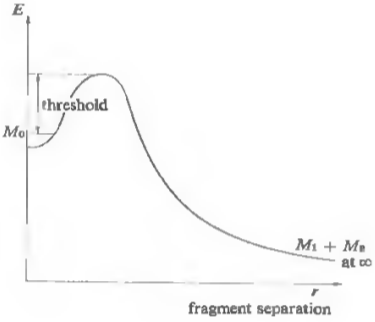
\includegraphics[width=\textwidth,height=0.5\textheight,keepaspectratio]{fissthre}
\caption{Energia di attivazione}
\label{fig:fissionthreshold}
\end{figure}


\begin{figure}[!ht]
\centering
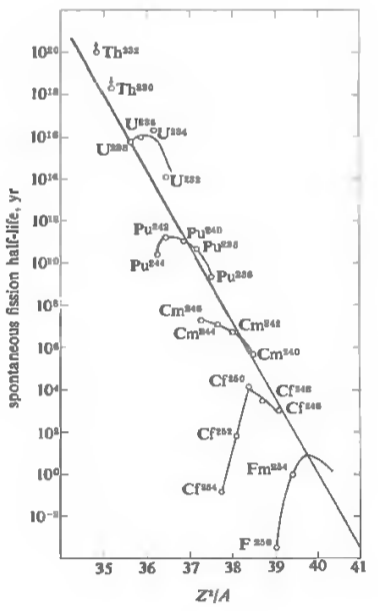
\includegraphics[width=\textwidth,height=(\textheight-20mm),keepaspectratio]{sfissionhalf}
\caption{Tempo di dimezzamento ($\thalf\propto\frac{1}{\lambda}$) per fissione spontanea: general trend of decreasing lifetime with incresing of $\frac{Z^2}{A}$.}
\end{figure}


\begin{figure}[!ht]
\centering
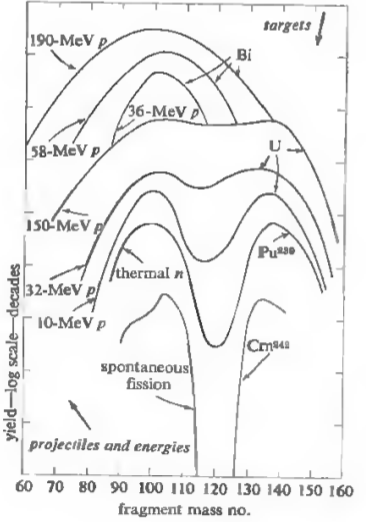
\includegraphics[width=\textwidth,height=(\textheight-11mm),keepaspectratio]{yieldvstypes}
\caption{Shape of mass distro: deps upon nature and energy.}
\end{figure}

\clearpage

\subsection{Emissione neutroni: nomenclatura.}
I frammenti di fissione sono ricchi di neutroni: si ha emissione di neutroni a $10^{-16}\,s$.

La probabilit\'a che siano emessi n neutroni \'e una gaussiana centrata in $\nu$, $\sigma\approx1.08$.

 Classifico i neutroni in base alla loro energia
 \begin{itemize*}
 \item Thermal: $E\approx0.025\,eV$.
 \item Epithermal: $E\approx1\,eV$.
 \item Slow: $E\approx1\,KeV$.
 \item Fast: $E\approx100\,KeV-10\,MeV$.
 \end{itemize*}

\subsection{Catena di decadimenti in seguito a fissione di $^{235}U$.}

Fission fragments produced in $^{235}U$ slow neutron fission that have excess of neutrons revert to stability by a succession of beta decay forming chain of isobar:

\begin{align*}
&_{54}Xe\xrightarrow{16\,s}_{55}Cs\xrightarrow{66\, s}_{56}Ba\xrightarrow{12.8\,d}_{57}Xe\xrightarrow{40\,h}_{58}Ce(\text{stable})&\intertext{questa sopra \'e la catena dei frammenti massivi $A=140$}\\
&_{40}Zr\xrightarrow{30 s}_{41}Nb\xrightarrow{3.8\,m}_{42}Mb\xrightarrow{67\,hr}_{43}Tc\xrightarrow{2.2*10^5\,yr}_{44}Ru(\text{Stable})&\intertext{Questa sopra \'e la catena dei frammenti leggeri con $A=99$.}
\end{align*}
\clearpage

\subsection{Energy release}
\begin{figure}[!ht]
\centering
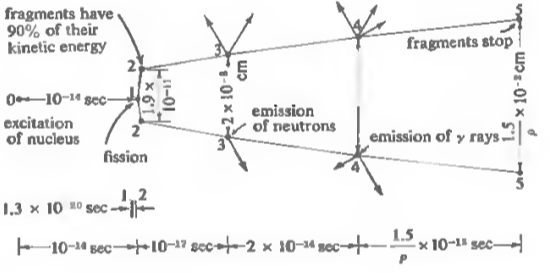
\includegraphics[width=\textwidth,height=(\textheight-11mm),keepaspectratio]{GraphisRfissionp}
\caption{Graphic representation of fission process}
\end{figure}

La fissione di $^{235}U$ libera $Q=200\,MeV$ che si distribuiscono
\begin{itemize*}
\item $\gamma$ rays: $7\,Mev$ from fragments, $8\,MeV$ immediatamente dopo la fissione.
\item $80\%$: Kinetic energy of fragments
\begin{equation*}
\frac{T_1}{T_2}=\frac{m_2}{m_1}\propto(\frac{A_1}{A_2})^{-1}
\end{equation*}
\item Prompt neutrons: $5\,MeV$
\end{itemize*}

\clearpage

\section{Q di fissione, energia di attivazione.}

\subsection{Processi di fusione.}

\begin{align*}
&^A_ZX_N\to^{A_1}_{Z_1}Y_{N_1}+^{A_1}_{Z_1}Z_{N_1}+k*n\\
&\tau\approx10^{-16}\,s\\
&n+^A_ZX_N\to^A_ZX_N^*\to^{A_1}_{Z_1}Y_{N_1}+^{A_1}_{Z_1}Z_{N_1}+k*n\\
&\tau\approx10^{-21}\,s
\end{align*}

Definisco $\nu=\exv{k}$ (per $^{235}U$ $\nu\approx2.4$)

Dalla curva della BE per nucleone vedo
\begin{itemize*}
\item L'energia liberata in un processo di fissione \'e 1 MeV per nucleone
\item Per nuclei con $A>56$ \'e energeticamente possibile
\end{itemize*}

\subsection{Q di fissione}

Stima rozza per fissione in 2 frammenti simmetrici:

$^A_ZX_N\to2^{\frac{A}{2}}_{\frac{Z}{2}}X_{\frac{N}{2}}$.

\begin{align*}
Q&=M(X)-2M(Y)=2B({\frac{A}{2}},{\frac{Z}{2}})-B(A,Z)\\
&\approx a_S(1-2^{\frac{1}{3}})A^{\frac{2}{3}}+a_C(1-2^{-\frac{2}{3}})\frac{Z^2}{A^{\frac{1}{3}}}\\
a_S&=18.56 Mev,\quad a_C=0.717 MeV
\end{align*}
da cui 
\begin{equation*}
Q>0\quad\Leftrightarrow\quad\frac{Z^2}{A}>18.2
\end{equation*}


\subsection{Barriera Coulombiana}
Fission doesn't compete succesfully with alpha decay:

per $^{238}U:\quad\thalf^{\alpha}=4.5*10^9 yr<\thalf^{fission}=10^{16} yr$.

Dalla barriera Coulombiana per lo splitting simmetrico di U-238 stimo l'altezza della buca di potenziale e dall'energia rilasciata (il Q-valore) l'energia delle due particelle nella buca

\begin{align*}
V=k_0\frac{Z_1Z_2e^2}{R}=1.44*MeV*fm*\frac{(46)^2}{12.2 fm}=250\, MeV\\
R=R_1+R_2=2*1.25*(119)^{\frac{1}{3}}=12.2\,fm
\end{align*}

\begin{figure}[!ht]
\centering
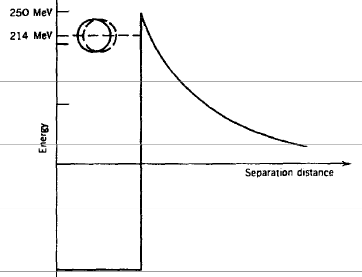
\includegraphics[width=\textwidth,height=(\textheight-70mm),keepaspectratio]{CoulombBU238}
\caption{Barriera Coulombiana per $^{238}U$}
\end{figure}

\clearpage

\subsection{Energia di attivazione}
\'E l'energia da fornire al nucleo per provocarne la fissione: la differneza tra l'energia del livello fondamentale senza deformazione e il livello pi\'u basso instabile per deformazione.
\begin{figure}[!ht]
\centering
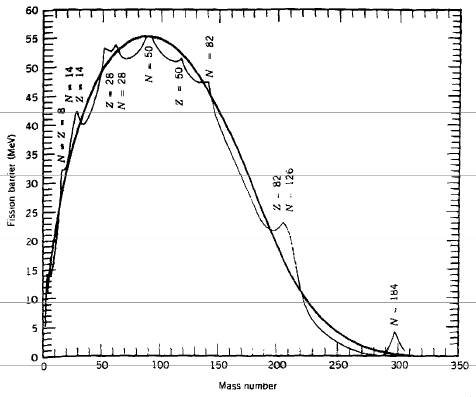
\includegraphics[width=\textwidth,height=(\textheight-11mm),keepaspectratio]{attener}
\caption{Energia di attivazione vs A}
\end{figure}

\clearpage

\section{A natural limit to stability of nuclei against spontaneous fission.}\label{sec:deformednucleus}

\subsection{Modello collettivo: nucleo stabile in forma non sferica}

In una configurazione a strati completi il nucleo \'e sferico, l'aggiunta di pochi nucleoni produce solo piccole deformazioni, per configurazioni con strati completi a met\'a i nuclei si discostano apprezzabilmente dalla forma sferica. I momenti di quadrupolo per nuclei in prossimit\'a di shell chiuse si accordano bene con il valore del quadrupolo di singola particella esterna, per shell piene a met\'a sono molto pi\'u grandi di quelli per particella singola.

Rainwater (1950) ha suggerito che la particella singola pu\'o deformare l'intero nucleo: i nucleoni si muovono in un potenziale non pi\'u a simmetria sferica.

Considero il core del nucleo contenente in nucleoni degli strati completi, al di fuori ci sono n nucleoni:
\begin{itemize*}
\item Per $n=\pm1$ il modello a shell si pu\'o applicare efficentemente.
\item Per $|n|>1$ e pari i nucleoni della nube sono soggetti a interazioni a corto raggio che orientano gli spin di coppie di nucleoni identici: forma sferica e spin nullo; sono presenti anche  componenti a lungo raggio che tendono a far sovrapporre tutte le autofunzioni delle n particelle: i nucleoni sono spinti in certe direzioni e il nucleo si deforma.
\end{itemize*}

\begin{align*}
H=\frac{p^2}{2m}+V_0(r)+V_2(r)P_2(\cos{\theta})+V_{so}\scap{l}{s}&\intertext{nucleo ellissoidale caratterizzato da $\Delta R/R=\delta$ con $V_2$ primo termine sviluppo in funzioni sferiche}
\end{align*}

Per nuclei deformati i i numeri magici differiscono da quelli per nucleo di forma sferica: i nuclei superpesanti sono instabili per fissione.

\subsection{Stabilit\'a per piccole deformazioni: Parametro di deformazione.}

\begin{align*}
R(\theta,\phi)=R_{av}[1+\beta Y_{20}(\theta,\phi)]&\intertext{descrive un ellissoide di rivoluzione}\\
\beta\propto\frac{\Delta R}{R}\propto\epsilon&\intertext{\'e il parametro di deformazione}
\end{align*}
Per $\beta(\beta_1,\ldots,\beta_q)=0$ ho il nucleo sferico.
Definisco la variazione di energia per deformazione ($c=1$)
\begin{equation*}
\Delta E=E(\beta)-E(0)=B(0)-B(\beta)
\end{equation*}

\begin{figure}[!ht]
\centering
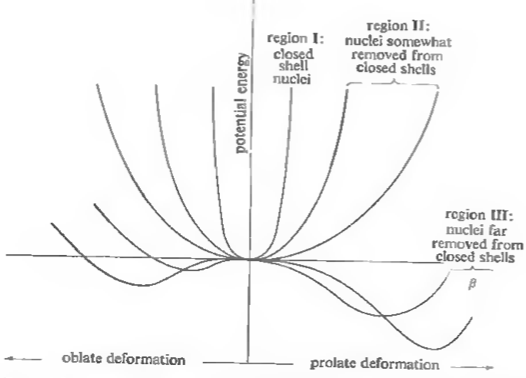
\includegraphics[width=\textwidth,height=0.5\textheight,keepaspectratio]{VvsDef}
\caption{Energia potenziale in funzione della deformazione e per diverse zone del chart di Segre.}
\end{figure}

\clearpage

\subsection{Coulomb repulsion vs surface tension for small deformation.}
Fatte le ipotesi
\begin{enumerate*}
\item Liquido incomprimibile
\item Distribuzione di carica costante ed uniforme
\item Rapporto $Z/N$ costante
\end{enumerate*}

esplicito $B(\epsilon)$ (con $\epsilon=\frac{2\Delta R}{3R})$:


$-\Delta B\to\Delta E$
\begin{align*}
&a=R_0(1+\epsilon)\quad b=\frac{R_0}{\sqrt{1+\epsilon}}&\intertext{per l'ellissoide.}
&E(\epsilon)-E(0)=[E_S(\epsilon)-E_S(0)]+[E_C(\epsilon)-E_C(0)]\\
&E_S(\epsilon)=\sigma S(\epsilon)\\
&E_C=\frac{1}{2}k_0\int_{V(\epsilon)}\frac{\rho(\vec{r_1})\rho(\vec{r_2})}{|\vec{r_1}-\vec{r_2}|}\,d^3r_1\,d^3r_2
\end{align*}

All'ordine pi\'u basso in $\epsilon$:

\begin{align*}
S(\epsilon)\approx4\pi R_0^2(1+\frac{2}{5}\epsilon^2)\\
B(0)-B(\epsilon)\approx(2a_SA^{\frac{2}{3}}-a_C\frac{Z^2}{A^{\frac{1}{3}}})\frac{\epsilon^2}{5}
\end{align*}

\subsection{Parametro di fissionabilit\'a: rapporto $Z^2/A$ critico}

\begin{equation*}
x=\frac{1}{2}\frac{E_C(0)}{E_S(0)}=\frac{a_C}{2a_S}\frac{Z^2}{A}
\end{equation*}

Definisco il rapporto $Z^2/A$ critico tale che $x=1$
\begin{align*}
x=1=\frac{1}{2}\frac{E_C(0)}{E_S(0)}=\frac{a_C}{2a_S}(\frac{Z^2}{A})\\
(\frac{Z^2}{A})_{crit}=\frac{2a_S}{a_C}\approx49
\end{align*}

\subsection{Stabilit\'a per piccole deformazioni}
\begin{align*}
\Delta E=B(0)-B(\epsilon)=2\frac{a_SA^{\frac{2}{3}}\epsilon^2}{5}(1-x)\\
E(\epsilon)-E(0)>0\quad\Leftrightarrow\quad x<1:\quad\frac{Z^2}{A}<(\frac{Z^2}{A})_{crit}\\
E(\epsilon)-E(0)<0\quad\Leftrightarrow\quad x>1:\quad\frac{Z^2}{A}>(\frac{Z^2}{A})_{crit}&\intertext{in quest'ultimo caso il nucleo \'e fissile.}
\end{align*}

\section{Mass distribution of fragments}

\subsection{Threshold yield distro}

\begin{figure}[!ht]
\centering
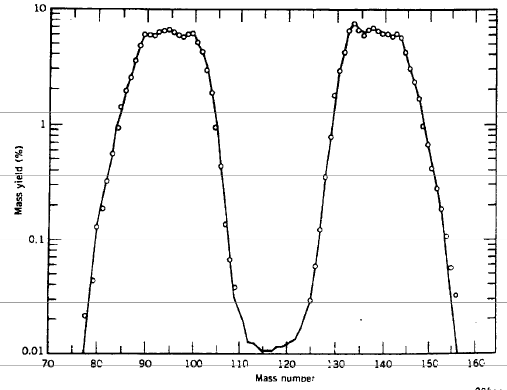
\includegraphics[width=\textwidth,height=(\textheight-11mm),keepaspectratio]{massyield}
\caption{Distribuzione frammenti di fissione per $^{235}U+n$ in soglia.}
\end{figure}

\clearpage

\subsection{Shell effects}
Nel gruppo dei frammenti pesanti (at lower edge) c'\'e il nucleo doppiamente magico $^{132}_{50}Sn_{82}$ mentre il gruppo dei frammenti leggeri non si sovrappone con  $N=50$: aumentando i nucleoni del nucleo fissile questi si aggiungono al frammento leggero.

\begin{figure}[!ht]
\centering
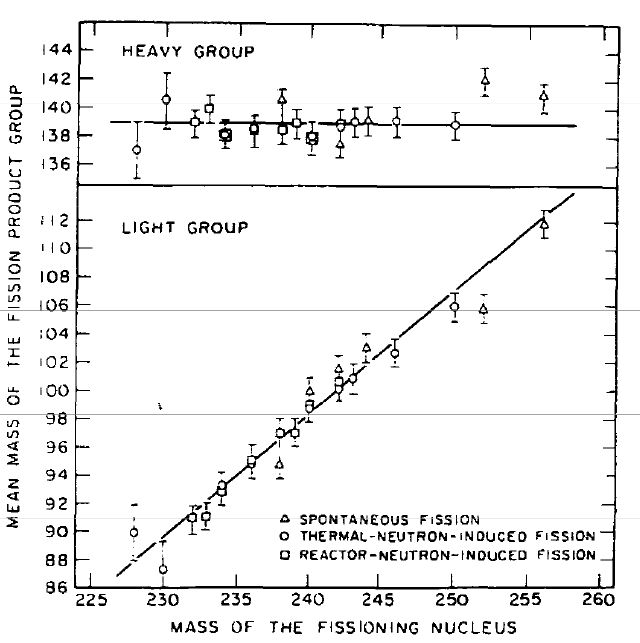
\includegraphics[width=\textwidth,height=(\textheight-60mm),keepaspectratio]{lHfrag}
\caption{Mean mass of fission product: lightand heavy fragments.}
\end{figure}


\section{Dependence of fission probability upon nuclear structure}

\subsection{Sezione d'urto per fissione indotta: $^{235}U$ e $^{238}U$.}

Threshold energy

La BE di un \Pneutron catturato da un nucleo con numero dispari di neutroni aumenta di  $0.8 \,MeV$ (livello fondamentale diminuito di $\delta$): l'energia di eccitazione \'e addizionata di un termine $\delta$ che non \'e presente nei nuclei con A dispari. Nel caso invece di cattura da parte di un nucleo con A pari ($^{238}_{92}U_{146}$) l'energia del livello fondamentale prima della cattura \'e diminuita del termine di pairing e l'energia di eccitazione di $^{A+1}X$ \'e diminuita di conseguenza.

un neutrone lento catturato da un nucleo con N dispari ($^{235}U\,^{239}Pu$)da vita ad un compound nucleus more excited by about $0.8\,MeV$ rispetto rispetto a quello che si avrebbe per cattura da un nucleo pari-pari ($^{238}U$).

\begin{itemize*}
\item Thermal region shows $\frac{1}{v}\quad(v=\sqrt{\frac{2E}{m}})$ dependence.
\item Resonances in $1-100\,eV$ region.
\item Different behaviour of $^{238}U/^{235}U$ fission cross section: Excitation energy of compound nucleus and activation energy.
\end{itemize*}
%fig11.140

\subsection{Effetto del termine di pairing}

\begin{itemize*}
\item $^{235}U$ capturing \Pneutron
\begin{align*}
E_{ex}&=[m(^{236}U^*)-m(^{236}U)]c^2\\
m(^{236}U^*)&=m(^{236}U)+m_n\\
&=235.0439\,u+1.00866\,u&\intertext{facendo le somme}\\
E_{ex}&=(236.052589\,u-236.045563\,u)\\
&\quad*931.5\,MeV/u=6.5\,MeV&\intertext{Exceeding the energy needed to excite $^{236}U$ into fissionable state ($6.2\,MeV$)}
\end{align*}

\item $^{238}U$ capturing \Pneutron
\begin{align*}
E_{ex}=4.8\,MeV&\intertext{minore dell'energia di attivazione per A+1 ch\'e}\\
6.6\,MeV
\end{align*}
\end{itemize*}

La spiegazione sta nella differnza di BE dovuta al termine di pairing:

%krane 491 fig 13.11
\begin{itemize*}
\item $^{236}U$ (that is $A+1$ nucleus) is increased by $\delta\approx0.56\,MeV$ (ground state lowered) and $E_{ex}$ is increased by $\delta$.
\item $^{238}U$ (that is $A$ nucleus) is increased by $\delta$ (ground state lowered) and the energy of captured state is corr. lowered: $E_{ex}$ is lowered by $\delta$ relative to its value without pairing term.
\end{itemize*}
The result is a difference in excitation energies between the 2 nuclei of $2\delta\approx1.1\,MeV$.

We expect odd-N nuclei will has larger thermal cross section than even-N nuclei.

\section{Isomeri di fissione}

\subsection{Effects of shell structure in fission barrier: doubled humped barrier.}

In realt\'a il livello fondamentale dei nuclei fissili spesso non \'e sferico: average non spherical potential that cause different position of levels.

The magic number for deformed nucleus may be not the same as for spherical nucleus.

L'energia di un nucleo varia in seguito a deformazione per 2 motivi
\begin{itemize*}
\item Surface and electrostatic effects give rise to average variation (smooth function of A)
\begin{equation*}
B(\epsilon)-B(0)\approx(-\frac{2}{5}a_sA^{\frac{2}{3}}+\frac{1}{5}a_CA^{-\frac{1}{3}})\epsilon^2
\end{equation*}

\item The shell effects produce fluctuations (dell'ordine del MeV) around the smooth value.
For some levels the energy increase for some decrease: if the valence nucleons are in states with positives slopes the energy increase in deformation will be a bit faster than the parabola (of point above) because the single particle energy also increase with $\epsilon$. At some point there will be a crossing between state of positive and negative slopes: the valence nucleons choosing lowest state we have oscillations in nuclear energy.
\end{itemize*}

\subsection{Fission probability and shape of barrier}
Posso distingure 3 tipi di fisione a seconda dello stato eccitato del nucleo di partenza
\begin{figure}[!ht]
\centering
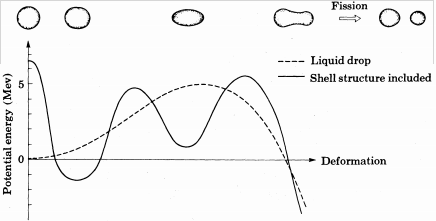
\includegraphics[width=(\textwidth-18mm),height=(\textheight-11mm),keepaspectratio]{doublehumppot}
\caption{Potential energy function for deformations leading to fission}
\end{figure}

\begin{itemize*}
\item From states in the continuum above threshold: $\tau\approx10^{-16}-10^{-20}\,s$.
\item From isomer states in the second well: $\tau\approx10^{-2}-10^{-9}\,s$.

Polikanov, 1962: $^{242}Am$, $^{240}Pu$.

These states are reached with $(n,\gamma)$, $(\alpha,2n)$ or other reactions: Frank-Condon principle.
\item Spontaneous fissions: $\thalf\approx\,hrs->10^9\,yr$
\end{itemize*}

\clearpage

\subsection{Isomeri di fissione e risonanze nella sezione d'urto}
There are many resonances in $eV-KeV$ region: fission resonances (under threshold) cluster into group.

\begin{itemize*}
\item States in first well are spaced about eV (density of states depends on excitation energy abouve ground state)
\item States in second well are speced about $0.1-1\,MeV$ and since have greater prob. to fission the have a greater width ($\Delta\tau\Delta E\geq\frac{\hbar}{2}$)
\end{itemize*}

The resonant fissioning states are selected through averlap in energy between the states in first and second well.

\begin{figure}[!ht]
\centering
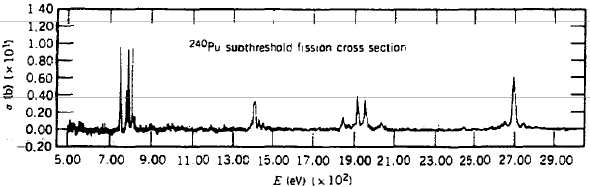
\includegraphics[width=(\textwidth-18mm),height=(\textheight-11mm),keepaspectratio]{fissres-pu240}
\caption{Fission cross section of Pu-240}
\end{figure}

\clearpage

\subsection{Experimental verif.}
Measurement of rotational spectra of excited states confirm this hypothesis: as deformation increses the moment of inertia becomes larger thus rotational states closer.

\section{Fissione controllata. Neutron physics.}

\subsection{Generazione di neutroni}
\begin{itemize*}
\item $\alpha-Be$ source: neutron energies spread over several MeV.

we mix of alfa emitter $^{226}Ra$(hystorical), $^{238}Pu$, $^{241}Am$, $^{210}Po$ and $^9Be$

\begin{equation*}
^4He+^9Be\to^{12}C+\Pneutron
\end{equation*}
Most probable energy is $5\,MeV$ and for each Ci of Ra are generated $10^7$ \Pneutron  
\item Photoneutron source (more monoenergetic).

$^{124}Sb$ emits gamma radiation above separation energy of berillium neutrons 
\begin{equation*}
\gamma+^9Be\to^8Be+\Pneutron
\end{equation*}

\item Fissione spontaneo.

Comunemente si usava il $^{252}Cf$ da cui si ottengono neutroni con energia media $1-3\,MeV$.

\item Other reactions.

\begin{align*}
^3H+d\to^4He+\Pneutron
^7Li+\Pproton\to^7Be+\Pneutron
^2H+d\to^3He+\Pneutron
\end{align*}

\item Reactors.
Nel core di un reattore a fissione abbiamo un flusso di neutroni di $10^{14}\Pneutron/s/cm^2$.

\end{itemize*}

\subsection{\Pneutron from fission.}

\begin{itemize*}
\item neutroni emessi durante la fissione (pronti).

\begin{figure}[!ht]
\centering
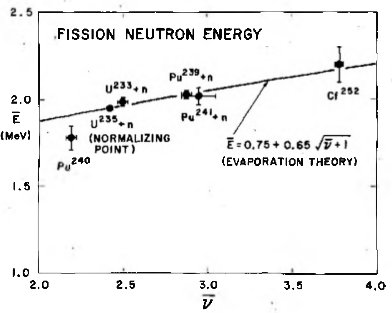
\includegraphics[width=(\textwidth-18mm),height=(\textheight-11mm),keepaspectratio]{Evsnum}
\caption{Energia media vs numero medio di \Pneutron pronti}
\end{figure}

\begin{figure}[!ht]
\centering
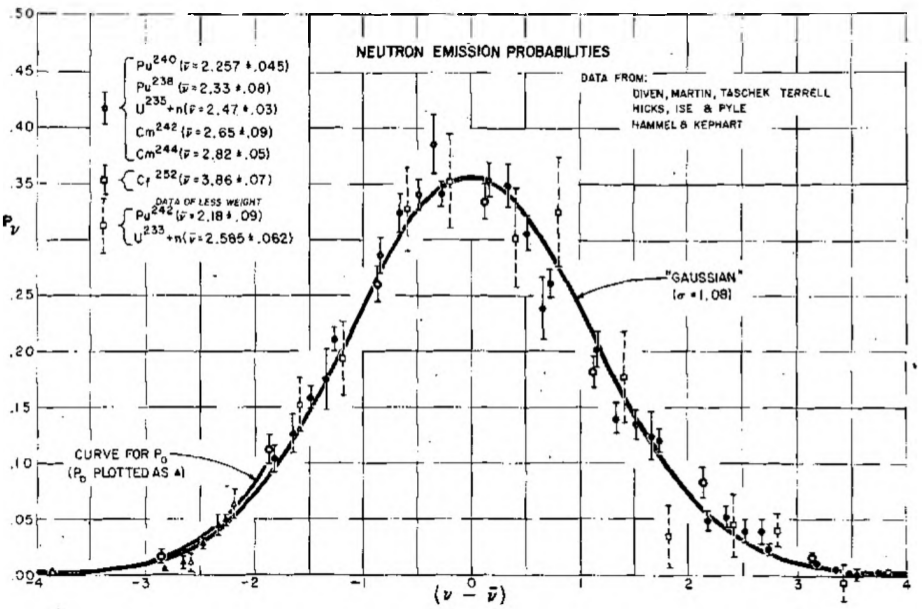
\includegraphics[width=(\textwidth-18mm),height=(\textheight-11mm),keepaspectratio]{nProb}
\caption{Probabilit\'a di emissione di n neutroni}
\end{figure}

\item Neutroni ritardati.

In seguito alla fissione i frammenti con eccesso di neutroni decadono beta $Z\to Z+1$ in uno stato eccitato di un isobaro: se l'energia di eccitazione \'e al di sopra dell'energia di legame del neutrone \'e probabile che un \Pneutron venga emesso.  

\end{itemize*}

\clearpage

\section{Sezione d'urto per fissioni indotte.}

\begin{figure}[!ht]
\centering
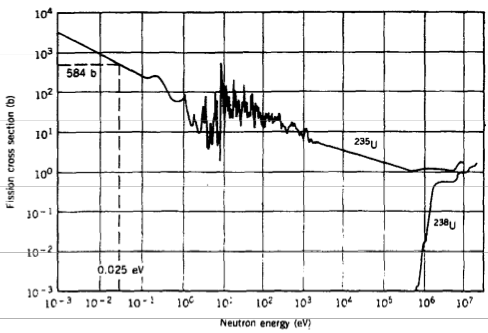
\includegraphics[width=(\textwidth-18mm),height=(\textheight-11mm),keepaspectratio]{U235-238}
\caption{Probabilit\'a di emissione di n neutroni}
\end{figure}


\subsection{Assorbimento neutroni veloci}
Danno luogo a una moltitudine di reazioni
\begin{itemize*}
\item $(\Pneutron,\Pproton)$
\item $(\Pneutron,\alpha)$
\item $(\Pneutron,2\Pneutron)$
\end{itemize*}

\subsection{Assorbimento neutroni lenti}
\begin{itemize*}
\item Capture reaction $(\Pneutron,\Pphoton)$.

Often dominated by large resonance, off resonance $\sigma_{a}\propto\frac{1}{v}$.
\end{itemize*}

\subsection{Sezione d'urto di fissione}
$^{235}U$ ha una sezione d'urto di fissione grande per neutroni lenti risultante dall'andamento $\frac{1}{v}$: $\sigma_{Fus}\approx580b$.

\clearpage

\section{Scheme of pile reactor: uranio e grafite.}

\subsection{Uranio naturale}
In natura \'e presente con la composizione: piccola percentuale di $^{235}U:\quad0.72\%$ radioattivo e il resto $^{238}U:\quad99.28\%$. 

\subsection{Neutron reproduction factor}
Nella fissione dell'uranio vengono rilasciati $200 MeV$ sotto forma di energia cinetica dei frammenti e radiazione e $2.5$ neutroni.

For infinite medium $k_{\infty}$ gives the net change in number of thermal neutrons from one generation to the next: on the average each thermal neutron produces $k_{\infty}$ thermal neutrons.

\subsection{Pila critica}
Perch\'e la reazione a catena continui deve essere $k_{\infty}>1$, la condizione $k_{\infty}=1$ \'e dette critica.

\subsection{Assorbimento vs fissione: U naturale}

\begin{align*}
\sigma_F=\frac{0.72}{100}\sigma_F(235)+\frac{99.28}{100}\sigma_F(238)=4.2b\\
\sigma_a=\frac{0.72}{100}\sigma_a(235)+\frac{99.28}{100}\sigma_a(238)=3.42b\\
\end{align*}

\subsection{Four factor formula}

\begin{enumerate*}
\item Fattore che tiene conto dei neutroni di fissione di U-235 e anche dell'assorbimento:

$\eta=\frac{\sigma_F}{\sigma_F+\sigma_a}$.

\item Fattore che tiene conto della fissione di U-238:

$\epsilon$ ($\epsilon\approx1.03$ per U-238 naturale).

\item Tengo conto della cattura risonante ($\sigma\approx10^4b$) nel range $10-100eV$ del U-238 tramite il fattore $P(\approx0.9)$.

\item Tengo conto della piccola sezione d'urto per assorbimento di neutroni lenti da parte del moderatore: f, the thermal utilization factor give the fraction of thermal neutron that are available to U-235,U-238.

\end{enumerate*}


\begin{equation*}
k_{\infty}=\eta\epsilon Pf
\end{equation*}

\section{Rallentamento dei neutroni.}

\subsection{Intensity of a beam: exponential law.}
Ogni neutrone di un fascio che attraversa uno spessore $dx$ di densit\'a numerica $n$ incontra $n\,dx$ particelle per unit\'a di superficie
\begin{equation*}
dI=-I\sigma_Tn\,dx\Rightarrow I=I_0\exp{-\sigma_Tnx}
\end{equation*}

\subsection{Relazioni tra la sezione d'urto nel CM e nel Lab.: Considerazioni cinematiche.}

\begin{itemize*}
\item Il momento totale nel sistema del centro di massa \'e zero.
\item Nel sistem CM il modulo della velocit\'a non cambia in un urto. I vettori sono ruotati dell'angolo di scattering $\theta_{CM}$.
\item La sezione d'urto \'e calcolata in CM ma si misura nel Lab.
\item L'energia cinetica totale misurata nel CM \'e minore di quella misurata nel Lab.: la differenza \'e l'energia dovuta al moto del CM.
\end{itemize*}

Definisco le grandezze che descrivono il problema di un urto di una particella leggera (massa di 1 nucleone) con un nucleo di massa A:
\begin{align*}
&(1+A)\vec{v_{CM}}=1*\vec{v_L}+A\vec{V_L}&\intertext{$\uparrow$ velocit\'a del CM (nucleo fermo).}\\
&\vec{v_C}=\vec{v_L}-\vec{v_{CM}}=\frac{A}{1+A}\vec{v_L}&\intertext{$\uparrow$ velocit\'a del neutrone nel sistema CM}\\
&\vec{V_C}=-\frac{1}{A+1}\vec{v_L}&\intertext{$\uparrow$ velocit\'a del bersaglio nel sistema CM}\\
&1*\vec{v_C}+A*\vec{V_C}=0&\intertext{$\uparrow$ momento totale nel sistema CM}\\
&E_L=\frac{1}{2}1*v_L^2\\
&E_C=\frac{1}{2}v_C^2+\frac{1}{2}AV_C^2=\frac{1}{2}\mu v_L^2&\intertext{$\uparrow$ the total kinetic energy in Lab. the former and in CM the latter}\\
\end{align*}

Conservazione del momento:
\begin{align*}
&v_C-AV_C=-AV_C'\cos{\theta_C}+v_C'\cos{\theta_C}\\
&0=-AV_C'\sin{\theta_C}+v_C'\sin{\theta_C}
\end{align*}

Ho le seguenti relazioni fra le velocit\'a dopo l'urto nel Lab e la velocit\'a del CM:

\begin{align*}
&H:\quad v_L'\cos{\theta_L}=v_{CM}+v_C'\cos{\theta_C}\\
&V:\quad v_L'\sin{\theta_L}=v_C'\sin{\theta_C}\\
&\tan{\theta_L}=\frac{v_C'\sin{\theta_C}}{v_{CM}+v_C'\cos{\theta_C}}=\frac{\sin{\theta}}{\frac{1}{A}+\cos{\theta_C}}&\intertext{quest'ultima lega $\theta_{CM}$ a $\theta_L$ discende dalle prime 2 e da $v_{CM}=\frac{1}{1+A}v_L$.}
\end{align*}

\begin{figure}[!ht]
\centering
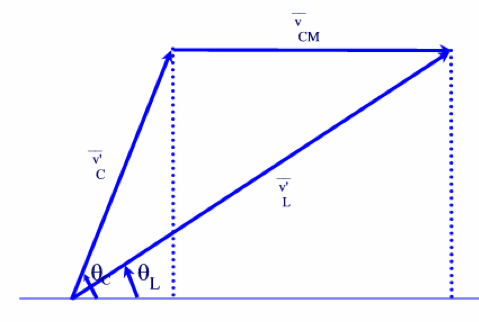
\includegraphics[width=\textwidth,height=0.3\textheight,keepaspectratio]{AnglesL-CM}
\caption{Angolo di scattering: CM e Lab}
\end{figure}

Relazione tra la sezione d'urto nel Lab. e nel CM:
\begin{align*}
\sigma_L(\theta_L)\sin{\theta_L}\,d\theta_L=\sigma_{CM}(\theta_C)\sin{\theta_C}\,d\theta_C\\
\sigma_L(\theta_L)=\sigma_{CM}(\theta_C)\frac{\sin{\theta_C}}{\sin{\theta_L}}\frac{d\theta_C}{d\theta_L}\\
\end{align*}

Ricavo $\frac{\sin{\theta_C}}{\sin{\theta_L}}$ e $\frac{d\theta_C}{d\theta_L}$:

\begin{align*}
&\frac{\sin{\theta_C}}{\sin{\theta_L}}=\frac{v_L'}{v_C'}=\frac{v_L'}{v_C}=\frac{v_L'}{\frac{A}{A+1}v_L}\\
&\frac{d\theta_C}{d\theta_L}=\frac{(\frac{1}{A}+\cos{\theta_C})^2}{\cos{\theta_L}^2(\frac{1}{A}\cos{\theta_C}+1)}&\intertext{$\uparrow$ questa sopra si ottiene differenziando l'equazione per $\tan{\theta_L}$. Esplicito $\cos^2{\theta_L}$ utilizzando H:}\\
&\cos{\theta_L}^2=(\frac{v_{CM}}{v_L'}+\frac{v_C'}{v_L'}\cos{\theta_C})^2=\frac{1}{(A+1)^2}\frac{v_C^2}{v_C'^2}(1+A\cos{\theta_C})^2&\intertext{sostituendo ho:}\\
&\frac{d\theta_C}{d\theta_L}=\frac{(\frac{1+A}{A})^2(\frac{v_L}{v_L'})^2}{\frac{1}{A}\cos{\theta_C}+1}
\end{align*}

Ricavo $(\frac{v_L'}{v_L})^2$:
\begin{align*}
&v_L'^2=v_{CM}^2+v_C'^2-2v_C'v_{CM}\cos{(\pi-\theta_C)}=v_C^2+v_C'^2+2v_C'v_{CM}\cos{\theta_{CM}}\\
&(\frac{v_L'}{v_L})^2=\frac{1+A^2+2A\cos{\theta_C}}{(1+A)^2}
\end{align*}

Scrivo la relazione esplicita
\begin{equation*}
\sigma_L(\theta_L)=\sigma_{CM}(\theta_C)\frac{(\frac{1}{A^2}+\frac{2}{A}\cos{\theta_C}+1)^{\frac{3}{2}}}{\frac{1}{A}\cos{\theta_C}+1}
\end{equation*}

\clearpage

\subsection{Rapporto energia tra finale e iniziale del neutrone.}

Come visto nel paragrafo sopra, ho:
\begin{equation*}
\frac{E'}{E}=\frac{v_L'^2}{v_L^2}=\frac{A^2+1+2A\cos{\theta_C}}{(A+1)^2}
\end{equation*}

Introduco il parametro di collisione $\alpha=(\frac{A-1}{A+1})^2$:
\begin{align*}
&1+\alpha=\frac{A^2+1}{(A+1)^2}\\
&1-\alpha=\frac{2A}{(A+1)^2}&\intertext{quindi riscrivo}\\
&E'=\frac{(1+\alpha)+(1-\alpha)\cos{\theta_C}}{2}E
\end{align*}

\subsection{Rallentamento per collisioni elastiche.}

I neutroni con energia minore di $1 MeV$ possono essere rallentati da collisioni elastiche.

In una collisione elastica fra neutroni con energia $E$ e velocit\'a $v$ con atomi a riposo di massa A l'energia finale del neutrone \'e:

\begin{align*}
&\frac{E'}{E}=\frac{A^2+1+2A\cos{\theta}}{(A+1)^2}\\
&\frac{E'}{E}=\frac{1}{2}[(1+\alpha)+(1-\alpha)\cos{\theta}]\\
&\alpha=(\frac{A-1}{A+1})^2\quad0\leq\alpha\leq1\\
&\underbrace{\alpha}_{\text{Max deflection:} \theta_{CM}=\pi}\leq\frac{E'}{E}\leq\underbrace{1}_{\text{No deflection:} \theta_{CM}=0}
\end{align*}

Per $\theta=\pi$ ho massimo trasferimento di energia:

$(\frac{E'}{E})_{Min}=(\frac{A-1}{A+1})^2$.

For low energy scattering we have isotropic distro in CM frame

\begin{align*}
&dw=p(\theta_{CM})\,d\theta_{CM}=\frac{d\Omega}{4\pi}\int\,d\phi=\frac{1}{2}\sin{\theta_{CM}}\,d\theta_{CM}\\
&dw=-P(E')dE'&\intertext{quindi}\\
&P(E')=-\frac{dw}{dE'}=-P(\theta_{CM})\frac{d\theta_{CM}}{dE'}=\frac{1}{E(1-\alpha)}&\intertext{Distribuzione di probabilit\'a per un neutrone scatterato con energia finale in $[E',E'+\,dE']$.}
\end{align*}

Parametro $\xi$.

\begin{align*}
&\xi=\exv{\log{\frac{E}{E'}}}=\frac{1}{4\pi}\int\log{\frac{(A+1)^2}{A^2+1+2A\cos{\theta}}}\,d\Omega\\
&(\xi=\frac{\int P(E')\ln{\frac{E}{E'}}\,dE'}{\int P(E')\,dE'})
\end{align*}

Il volore medio di $\log{E'}$ \'e diminuito dopo ogni urto di una quantit\'a $\xi$:
\begin{equation*}
\log{E'_n}=\log{E}-n\xi
\end{equation*}

Per rallentare un neutrone di fissione ($\approx2Mev$) a energie termiche sono necessari circa 110 urto nel caso il moderatore sia $^{12}C$.

\subsection{Thermal equilibrium distro}

Dopo un numero sufficiente di urti i neutroni raggiungono l'equilibrio termivo con il moderatore,  sia n il numero di neutroni per unit\'a di volume:

\begin{align*}
f(v)=4\pi n(\frac{m}{2\pi KT})^{\frac{3}{2}}v^2\exp{\frac{mv^2}{2KT}}\\
f(E)=\frac{2\pi n}{(2\pi KT)^{\frac{3}{2}}}E^{\frac{1}{2}}\exp{\frac{-E}{KT}}
\end{align*}